\documentclass[a4paper]{article}
% The website and PDF use the project's small, LaTeXML-compatible preamble.
% The original kod.sty remains beside this manuscript as the author's source
% style, but its tcolorbox/expl3 stack is not understood by LaTeXML.
\usepackage{mmp}
\usepackage{float}
\usepackage{mathtools}

\DeclarePairedDelimiter\abs{\lvert}{\rvert}%
\DeclarePairedDelimiter\norm{\lVert}{\rVert}%

\makeatletter
\let\oldabs\abs
\def\abs{\@ifstar{\oldabs}{\oldabs*}}
%
\let\oldnorm\norm
\def\norm{\@ifstar{\oldnorm}{\oldnorm*}}
\makeatother


%%%%%%%%%%%%%%%%%%%%%%%%%%%%%%%%%%%%%%%%%%%%%%%%%%

\title{\vspace*{10mm}\bf Polynomial moving points and lines on the plane and an olympiad geometry problem solving method} % Cím vagy téma ide

\author{Molnár-Szabó Vilmos\\ Bsc 2. year\\ \href{mailto:m.sz.vilmos@gmail.com}{m.sz.vilmos@gmail.com}\\ Supervisor: Frenkel Péter\\associate professor} % Szerző neve és email címe ide

\date{} % MARADJON ÜRESEN
%%%%%%%%%%%%%%%%%%%%%%%%%%%%%%%%%%%%%%%%%%%%%%%%%%

% Új parancs létrehozása: \newcommand{\parancs}{mit írjon ki}

% A híres számhalmazok parancsai az adott kisbetű kétszer, például a természetes számok halmaza \nn

\newcommand{\ord}{\operatorname{ord}}
\newcommand{\cdist}{\operatorname{cdist}}
\newcommand{\edist}{\operatorname{edist}}

%%%%%%% START %%%%%%%%%%

\begin{document}

\maketitle



%%%%%%%%%%%%%%%%%%%%%%%%%%%%%%%%%%%%%%%%%%%%%%%%%%
\section{Introduction}
The \textit{Method of Moving Points} or \textit{Animation} is an olympiad geometry problem solving method, that can be applied to more than half of the geometry problems in my experience, often solving them faster than the intended solution. People have been using it in several contests (including the IMO), even though the theorems in this topic aren't proved precisely. This paper aims to build a precise environment, prove the fundemental and some own theorems of this method and set up the concept of the 'square root' type method, which can solve a broader range of problems than the original method.


This is a quite fresh method, it was introduced in 2019, only proving the weaker versions of the theorems over $\rr$ instead of $\cc$ (giving only upper bounds for degrees).\cite{mmp}\cite{animation}



I proved that the upper bounds for degrees are strict, and for that reason I had to deal with multiplicities, and points at infinity, so I used the standard charts of $\cc\pp^n$ to define local coordinates even at points at infinity. I defined polynomial moving points in a more symmetric way by bivariate homogeneous polynomials. With this definition I could give clear, and short proofs to the fundamental theorems.

When the geometry problem contains an intersection of a line and a conic, the two intersection points' coordinates aren't polynomial, instead a square root of a polynomial appears in them. Since I came across many such problems, I made the square root extension of the method, which is discussed in the second half of my paper. I built up a more general environment to handle these points, and generalized almost every theorem in the first half in this setting.

This method is fairly unknown, and as far as I know these are the only new results until now. I reached out to one of the authors who invented the method, and he also thought about some further ideas, basically on the same path as I did.


Lots of ideas are credited to my supervisor Frenkel Péter.



\section{Moving objects}

\subsection{The space we are working in}

We work in $\cc\pp^n$ with the standard complex structure. We are especially interested in $\cc\pp^2$, and we consider moving points, lines and conics in this space.

\subsection{Moving points}

We call a function $P: \cc\pp^1 \to \cc\pp^n$ a \textit{moving point}. We imagine it as if $\cc\pp^1$ was time, and $P(t)$ was the moving point.

We call $p(t,s)$ a \textit{polynomial of time} if it is a homogeneous bivariate polynomial. The intuition is that time is $\pp^1$, and it is denoted with homogeneous coordinates $(t:s)$. Therefore we can imagine $p$ as a single "time" variable polynomial.

A moving point $P$ is \textit{polynomial} if there exist degree $d$ polynomials of time $p_0,...,p_n$ with no common zero except $(0,0)$ such that $$P\bigl((t:s)\bigr)=\bigl(p_0(t,s):\ldots:p_n(t,s)\bigr)$$

with homogeneous coordinates.

The common degree $d$ of $p_0,\ldots,p_n$ is called the \textit{degree} of the polynomial moving point.

\begin{lemma}[The polynomials are unique up to a constant multiplier]
\hfill\break
    If we have $p_0,...,p_n, q_0,...,q_n \in \cc[t,s]_h$ with no common zeros except the origin, such that
    $$P(t)=(p_0(t,s):...:p_n(t,s))=(q_0(t,s):...:q_n(t,s))$$
    then $\exists \lambda \ne 0 \in \cc$: $ (p_0,...,p_n)=\lambda(q_0,...,q_n) $
\end{lemma}

\begin{proof}
    Since $(p_0(t):...:p_n(t))=(q_0(t):...:q_n(t)) \quad \forall t,s\ne\infty$
    $$\frac{p_0(t)}{q_0(t)}=...=\frac{p_n(t)}{q_n(t)}=\frac{a(t)}{b(t)}$$
    where $a,b\in \cc[t,s]_h$ are relatively prime polynomials.

    $\forall i \quad \frac{p_i}{q_i}=\frac{a}{b} \implies p_ib=q_ia \implies a\mid p_i$ and $b\mid q_i \implies a$ is a common factor of all $p_i$, but they don't have any, therefore $a$ is constant, and so is $b$ similarly. Neither $a$ nor $b$ is constant zero, and therefore $\lambda=\frac{a}{b}\ne 0\in \cc$ satisfies $(p_0,...,p_n)=\lambda(q_0,...,q_n)$.
\end{proof}

% \begin{lemma}
%     A polynomial moving point is holomorphic.
% \end{lemma}

% \begin{proof}
% \hfill\break

% Changing from homogeneous coordinates to local coordinates of the charts, and the other way round only use division. Therefore the mapping $$P(t:s)=(p_0(t,s):\ldots:p_n(t,s))$$ defined by homogeneous coordinates is also holomorphic in local coordinates.


% $P: \cc\pp^1 \to \cc\pp^n$ is a polynomial moving point. To prove that $\Omega$ is holomorphic in every $t$, we take a suitable chart in both $t \in \cc\pp^1$ and $\Omega(t) \in \cc\pp^n$.

% $t\ne \infty$ case:
% $\Omega(t)=(p_0(t):...:p_n(t))$

% $\exists i \quad p_i(t)\ne 0$

% According to the $i$-th chart $\Omega(t)=(p_0(t):...:p_n(t))=\left(\frac{p_0(t)}{p_i(t)},...,1,...,\frac{p_n(t)}{p_i(t)}\right)$, and rational functions are holomorphic.

% $t= \infty$ case:
% We have to check if $\Omega(\frac{1}{t})$ is holomorphic at $t=0$.

% \begin{equation*}
%    \Omega \left(\frac{1}{t}\right)=
%     \begin{cases}
%       (p_0(\frac{1}{t}):...:p_n(\frac{1}{t})) & t\ne 0 \\
%       (a_{d,0}:...:a_{d,n}) & t=0
%     \end{cases}
%     =
% \end{equation*}
% \begin{equation*}
%     =
%     \begin{cases}
%       (a_{d,0}(\frac{1}{t})^d+...+a_{0,0}:...:a_{d,n}(\frac{1}{t})^d+...+a_{0,n}) & t\ne 0  \qquad /\cdot t^d \\
%       (a_{d,0}:...:a_{d,n}) & t=0
%     \end{cases}
% \end{equation*}
% \begin{equation*}
%     =(a_{d,0}+...+a_{0,0} t^d:...:a_{d,n}+...+a_{0,n} t^d)=(p_0^*(t),...,p_n^*(t))
% \end{equation*}
% Since $d$ is the degree of the moving point, it is the maximum degree of $p_i$-s, so $\exists a_{d,i}\ne 0 \implies p_i^*(0)\ne 0$, so taking the i-th chart on $\cc\pp^n$, we have to divide everything by $p_i^*$, and rational functions are holomorphic.

%\end{proof}

\subsection{Moving lines}

We are now in $\cc\pp^2$, however the things mentioned here can be generalised to hyperplanes in $\cc\pp^n$.

A projective line is defined by its homogeneous coordinates, just like points. A polynomial moving line and its degree are defined the same way as for a polynomial moving point:

A moving line $e(t:s)=(p_1(t,s):p_2(t,s):p_3(t,s))$ is a \textit{polynomial} moving line, where $p_0,p_1,p_2$ are degree $d$ polynomials of time with no common zeros except $(0,0)$, and the common degree $d$ is the \textit{degree} of the polynomial moving line.

\subsection{Moving conics}
We can define the degree of a moving conic too. Conics are uniquely determined by their 6 coefficients up to homogeneity, so a conic corresponds to a point in $\cc\pp^5$:

$$\{Ax^2+Bxy+Cy^2+Dxz+Eyz+Fz^2=0\} \leftrightarrow (A:B:C:D:E:F)$$

A moving conic is \textit{polynomial} if it corresponds to a polynomial moving point in $\cc\pp^5$.

The \textit{degree} of the polynomial moving conic is the degree of its corresponding point.

We only consider the moving conics which are not always degenerate.

\subsection{Time-dependent quantities}

We can also define the degree of a quantity too, for example area of a triangle, the power of a point w.r.t. a circle, distances and (tangent of) angles.

These numbers correspond to a point in $\cc\pp^1$, so a polynomial quantity has a corresponding polynomial moving point in $\cc\pp^1$. The degree of the quantity is the degree of this moving point.


\section{Distances and areas in the complex plane}
We are in $\cc^2$.

The euclidean distance of two points $(p_1,p_2)$ and $(q_1, q_2)$ is
$$|PQ|=\sqrt{\abs{p_1-q_1}^2+\abs{p_2-q_2}^2}$$
This is a non-negative real number.



The euclidean distance of a point $P=(p_1,p_2)$ and a line $l:Ax+By+C=0$ is
$$\operatorname{dist}(P,l)=\frac{\abs{Ap_1+Bp_2+C}}{\sqrt{\abs{A}^2+\abs{B}^2}}$$

Twice of the euclidean area of the triangle formed by points $P=(p_1,p_2)$, $Q=(q_1, q_2)$ and $R=(r_1,r_2)$ is
$$\operatorname{area}(PQR\Delta)=\abs{
    \begin{vmatrix}
    p_1 & p_2 & 1\\
    q_1 & q_2 & 1\\
    r_1 & r_2 & 1
    \end{vmatrix}}$$
\begin{lemma}
    $2\cdot \operatorname{area}(PQR\Delta)=dist(P,QR)\cdot dist(QR))$
\end{lemma}
Since the line through $(p_1,p_2)$ and $(q_1, q_2)$ is $(A,B,C)=(p_1,p_2,1)\times (q_1, q_2,1)$,

$$\abs{
    \begin{vmatrix}
    p_1 & p_2 & 1\\
    q_1 & q_2 & 1\\
    r_1 & r_2 & 1
    \end{vmatrix}}
    =\abs{(p_1,p_2,1)\times (q_1, q_2,1) \cdot (r_1,r_2,1)}=\abs{(A,B,C)\cdot (r_1,r_2,1)}=\abs{Ar_1+Br_2+C}=$$
    $$=\frac{\abs{Ac_1+Bc_2+C}}{\sqrt{\abs{A}^2+\abs{B}^2}}\cdot \sqrt{\abs{A}^2+\abs{B}^2}=\frac{\abs{Ar_1+Br_2+C}}{\sqrt{\abs{A}^2+\abs{B}^2}}\cdot \sqrt{\abs{p_2-q_2}^2+\abs{q_1-p_2}^2}=\operatorname{dist}(P,QR)\cdot |QR|$$



The complex distance of two points $P=(p_1,p_2)$ and $Q=(q_1, q_2)$ is
$$\pm\sqrt{(p_1-q_1)^2+(p_2-q_2)^2}$$
This is a complex number along with its negative.

If line $PQ$ has slope $i$ or $-i$, this distance is zero, which is pretty awkward, so in the future we try to ban slope $i$ and $-i$ lines when calculating distances.

\begin{lemma}[Technical]
    For every $\epsilon>0$ there exists a $c>0$ such that if line $PQ$ has slope $s\in \cc$ with $|s-i|>\epsilon$ and $|s-(-i)|>\epsilon$, then
    $$c\cdot \operatorname{edist}(P,Q)\le |\operatorname{cdist}(P,Q)|\le \operatorname{edist}(P,Q)$$
\end{lemma}
\begin{proof}
    The second inequality says $|x^2+y^2|\le |x^2|+|y^2|$, which is triangle inequality.

    Let vector $PQ=(x,y)\in \cc^2$, and $s=\frac{y}{x}$. We can multiply both x,y with the same complex number, this doesn't change the statement, nor $s$, so we can assume $x=1$. ($x=0$ is trivial)

    Then we know $s=\frac{y}{x}=y$ is at least $\epsilon$ away from both $i$ and $-i$. Then since $z^2:\cc \mapsto \cc$ is an open map, there exists a $\delta>0$ such that $|y^2-(-1)|>\delta$ for every $y$ at least $\epsilon$ away from $i$ and $-i$. Set $c:=\operatorname{min}\{\frac{\delta}{3},\frac{1}{3}\}$.

    First assume $|y^2|<2$, then
    $$\frac{|\operatorname{cdist}(P,Q)|}{\operatorname{edist}(P,Q)}=\frac{|1+y^2|}{1+|y^2|}\ge \frac{\delta}{3}\ge c$$

    Now assume $|y^2|\ge2$:

    $$\frac{|\operatorname{cdist}(P,Q)|}{\operatorname{edist}(P,Q)}=\frac{|1+y^2|}{1+|y^2|}\ge \frac{1}{3}\ge c$$

\end{proof}

\begin{lemma}[Complex power of point]
    Let $P$ be a finite point, and $c$ a circle. Let $l$ be a line through $P$ with slope NOT $i$ or $-i$, and let $l$ intersect the circle in points $A$ and $B$. Then
    $\operatorname{cdist}(P,A)\cdot \operatorname{cdist}(P,B)$
    is the same for every such $l$.
\end{lemma}
\begin{proof}
    Let $p=(x_0,y_0,1)$ denote the homogeneous coordinates of $P$, and let the direction of $l$ be $(m,n)\in \cc^2$. Then the ideal point of $l$ has homogenous coordinates $v=(m,n,0)$. Then $l$ can be parametrized by homogeneous coordinates $p+tv$ for $t\in \cc$.

    Find the product of the two $t$-values for which $p+tv$ is on circle $c:x^TMx=0$, where $M\in \cc^{3x3}$ with the top left 2x2 submatrix is identity (this makes a conic circle).

    $$(p+tv)^TM(p+tv)=(v^TMv)t^2+(p^TMv)t+(p^tMp)=0$$

    The product of the two roots $t_1$ and $t_2$ is $t_1t_2=\frac{p^TMp}{v^TMv}$ by Viete formula. Note that $v^TMv=m^2+n^2$, where $v=(m,n,0)$, and this is nonzero, since $l$ does not have slope $i$ or $-i$.

    Now $\operatorname{cdist}(P,A)=t_1\sqrt{m^2+n^2}$ and $\operatorname{cdist}(P,B)=t_2\sqrt{m^2+n^2}$, so

    $$\operatorname{cdist}(P,A)\cdot \operatorname{cdist}(P,B)=t_1t_2(m^2+n^2)=\frac{p^TMp}{v^TMv}(m^2+n^2)=p^TMp$$

Therefore the power of point does not depend on the choice of $l$.
\end{proof}

$\ord_{t_0}(f)$ denotes the order of zero of $f$ at $t_0$, where $f$ can be one of several things:
\begin{itemize}
    \item a holomorphic function
    \item a function $\cc^n \mapsto \rr^+$ which lies in the generated subring of $\{\text{absolute value of holomorphic }\cc^n \mapsto \cc \text{ functions}\}$. In this case the order is the unique $\alpha \in \nn$ for which $\lim_{t\to t_0}\frac{f(t)}{|t-t_0|^\alpha}\to c$, where $c$ is a positive real number.
    \item a vector-valued function, in which case we take the minimum of the order of zeros of the coordinate functions, or equivalently the order of zero of the length of the vector.
    \item a bivariate homogeneous function, in which case for any $t\in \cc\pp^1$ we fix a nonzero coordinate in the homogeneous coordinate form of $t$, and take the order of zero of $f$ in the other coordinate.
\end{itemize}

$\ord(f)$ denotes the order of zero of $f$ at a point, where it is clear, which point we are talking about.

\begin{theorem}
    Let $P$, $A$, $B$, $C$, $D$ be polynomial moving points and $c$ be a polynomial moving conic such that $P$, $A$, $B$ are always collinear, and $P$, $C$, $D$ are always collinear too, and $A$, $B$, $C$, $D$ lie on $c$. Furthermore at a time $t_0$ all points are finite and $c$ is nondegenerate. Then
    $$\ord_{t_0}(\edist(P,A))+\ord_{t_0}(\edist(P,B))=\ord_{t_0}(\edist(P,C))+\ord_{t_0}(\edist(P,D))$$
\end{theorem}
\begin{proof}
    % First of all if lines $PA$ or $PC$ has slope $i$ or $-i$ at $t_0$, then apply an affine transformation so that this is no longer true. This does not change orders, nor the conditions of the theorem.

    Similarly to the previous proof, at a time $t$ let $v=(m,n,0)$ be the ideal point of $PA$, and $p=(x_0,y_0,1)$ be the homogeneous coordinates of $P$.
    Unlike in the previous proof, we care about euclidean distance, which is
    $$\operatorname{edist}(P,A)=|t_1|\sqrt{|m|^2+|n|^2} \text{ and }\operatorname{cdist}(P,B)=|t_2|\sqrt{|m|^2+|n|^2}$$

    Then

    $$\operatorname{edist}(P,A)\cdot \operatorname{edist}(P,B)=|t_1t_2|(|m|^2+|n|^2)=\frac{|p^TMp|}{|v^TMv|}(|m|^2+|n|^2)$$

    Since everything is moving polynomially, the coordinates of $v$, $M$ are changing continuously.

    At $t_0$ the ideal points of $PA$ and $PC$ are not on $c$, since $A$, $B$, $C$, $D$ are all finite, and $c$ is nondegenerate. Therefore at $t_0$ $v^TMv\ne 0$, and $(|m|^2+|n|^2)\ne 0$ since the homogeneous coordinates of $v$ can't be all zero. This implies that there exists $\epsilon>0$ and $M>0$, so that in a neighborhood around $t_0$ we know that $\epsilon<|v^TMv|<M$ and $(\epsilon<|m|^2+|n|^2<M)$.

    This means that in a neighborhood of $t_0$
    $$\frac{\epsilon^2}{M^2}<\frac{\operatorname{edist}(P,A)\cdot \operatorname{edist}(P,B)}{\operatorname{edist}(P,C)\cdot \operatorname{edist}(P,D)}<\frac{M^2}{\epsilon^2}$$

    Therefore

    $$\ord_{t_0}(\edist(P,A))+\ord_{t_0}(\edist(P,B))-\ord_{t_0}(\edist(P,C))+\ord_{t_0}(\edist(P,D))=$$
    $$=\ord_{t_0}\left(\frac{\operatorname{edist}(P,A)\cdot \operatorname{edist}(P,B)}{\operatorname{edist}(P,C)\cdot \operatorname{edist}(P,D)}\right)=0$$
\end{proof}

\begin{remark}
    Every theorem concerning orders works for square root objects too, since locally their coordinates can be written as a Puiseux series of time, and then we can define order to be a half integer, and everything works the same.
\end{remark}


\begin{definition}
    There are three points $A$, $B$ and $C$ in $\cc^2$ with lines $AB$, $AC$ having slope not equal to $i$ or $-i$. Let $AB=(x,y)$ and $AC=(z,v)$. Then the angle at $A$ is defined as
    $$\angle BAC=\pm \sin^{-1}\left(\frac{xv-yz}{\sqrt{x^2+y^2}\sqrt{z^2+v^2}}\right) \mod 2\pi$$
    For real valued points this gives back the normal angle definition.
\end{definition}

\begin{lemma}[Complex sine theorem]
    There are three points $A$, $B$ and $C$ in $\cc^2$ with lines $AB$, $BC$, $CA$ not having slope $i$ or $-i$. Then
    $$\frac{\cdist(A,B)}{\cdist(A,C)}=\pm\frac{\sin(ACB)}{\sin(ABC)}$$
\end{lemma}
\begin{proof}
    Let $AB=(x,y)$ and $AC=(z,v)$, and $CB=(x-z,y-v)$
    $$\frac{\cdist(A,B)}{\cdist(A,C)}=\frac{\sqrt{x^2+y^2}}{\sqrt{z^2+v^2}}=\frac{\frac{z(y-v)-v(x-z)}{\sqrt{z^2+v^2}\sqrt{(x-z)^2+(y-v)^2}}}{\frac{x(y-v)-y(x-z)}{\sqrt{x^2+y^2}\sqrt{(x-z)^2+(y-v)^2}}}=\frac{\sin(ACB)}{\sin(ABC)}$$
\end{proof}

\begin{lemma}
    There are three points $A$, $B$ and $C$ in $\cc^2$, and suppose at a time $t_0$ lines $AB$, $BC$, $CA$ do not have slope $i$ or $-i$, furthermore at $t_0$, $\angle BAC=0$, and $\angle ABC\ne 0$. Then
    $$\lim_{t\to t_0}\frac{\edist(A,B)}{\edist(B,C)}=0$$
    $$\lim_{t\to t_0}\frac{\edist(A,C)}{\edist(B,C)}=0$$
    $$\lim_{t\to t_0}\frac{\edist(A,C)}{\edist(A,B)}=1$$
\end{lemma}
\begin{proof}
    sine thm+technical lemma stating ratio of edist and |cdist| converge to a positive real number
\end{proof}























\section{Multiplicities}
To state any theorems, we have to define several types of multiplicities. Some multiplicites have an algebraic and a geometric definition, which are equivalent.



$a_1,...,\widehat{a_i},...$ means that $a_i$ is omitted from the sequence/sum.

% \begin{definition}
%     The homogeneous coordinates $(a_1(t):a_2(t):a_3(t))$ of the moving point $A(t)$ are \textit{right format} at some $t$ if all $a_i$-s are holomorphic at $t$ and not all $a_i(t)$-s are zero.
% \end{definition}

\textbf{1. point-point multiplicity:}

When two moving points, $A$ and $B$ coincide, this can happen with multiplicity.
The multiplicity of the coincidence is $\ord\bigl((A-B)\bigr)$ at the time of the coincidence. To calculate the derivatives, we use a chart containing the coincidency point.

For example, if at some time $A$ and $B$ are the same, and their derivative vector is the same, they coincide with at least mul. 2.

\begin{proof}
    Taking two different charts we get the same result:

    The transition map is holomorphic with nonsingular Jacobi-matrix, so by the p-p multiplicity lemma ~\ref{ppmul} (see later) we know that the two multiplicities are the same.
\end{proof}

\textbf{1' geometric definition:}

When two moving points, $A$ and $B$ coincide, this can happen with multiplicity.
The multiplicity of the coincidence is the order of zero of the euclidean distance of $A$ and $B$. To calculate the distance, we use a chart containing the coincidence point.

\textbf{1'' homogeneous definition:}

When two moving points, $A$ and $B$ coincide, this can happen with multiplicity.
The multiplicity of the coincidence is the order of zero of $(a_0,a_1,a_2)\times (b_0,b_1,b_2)$ where $(a_0,a_1,a_2)$ and $(b_0,b_1,b_2)$ are polynomial formats of $A$ and $B$.

\begin{proof}
    (1), (1') and (1'') are equivalent definitions:

    (1)$\iff$(1'):
    $$\ord\left(dist(A,B)\right)=\ord\left(\sqrt{\abs{a_1-b_1}^2+\abs{a_2-b_2}^2}\right)=\frac{1}{2} min\Bigl(\ord\bigl(\abs{a_1-b_1}^2\bigr),\ord\bigl(\abs{a_2-b_2}^2\bigr)\Bigr)=$$
    $$=min\Bigl(\ord\bigl(\abs{a_1-b_1}\bigr),\ord\bigl(\abs{a_2-b_2}\bigr)\Bigr)=min\Bigl(\ord\bigl(a_1-b_1\bigr),\ord\bigl(a_2-b_2\bigr)\Bigr)=\ord\bigl((a_1-b_1,a_2-b_2)\bigr)=\ord\bigl((A-B)\bigr)$$

    (1)$\iff$(1''):

    $A$ and $B$ coincide on the i-th chart. We can suppose that the i-th coordinate of both $a=(a_1,a_2,a_3)$ and $b=(b_1,b_2,b_3)$ is 1, because we can divide all coordinates by the actual i-th coordinate, which is a nonzero,
    holomorphic function, so it doesn't affect the order of $a\times b$, which is bilinear in $a$ and $b$. Let $h=b-a$. $a\times b=a\times (a+h)=a\times a+a\times h=a\times h$. Just for the sake of easy reading, suppose that i=3. Then $a=(a_1,a_2,1)$ and $h=(h_1,h_2,0)$, so $a\times h=(-h_2,h_1,a_1h_2-a_2h_1)$.
    It follows that $\ord(a\times b)=\ord(a\times h)=min(\ord(-h_2),\ord(h_1),\ord(a_1h_2-a_2h_1))=min(\ord(h_2),\ord(h_1))=\ord((h_1,h_2))=\ord((a_1-b_1,a_2-b_2))$

\end{proof}

\textbf{2. point-line multiplicity:}\label{plmul}

If a point $P$ lies on hyperplane (line) $l$ at a time $t_0$, this can happen with multiplicity. The multiplicity of this is
$$\ord_{t_0}\big((l_1,...,l_{n+1})\cdot (p_1,...,p_{n+1})\big)$$
where $(l_1:...:l_{n+1})$ and $(p_1:...:p_{n+1})$ are polynomial formats of $l$ and $p$.

\textbf{2' geometric definition:}

If a point $P$ lies on line $l$, this can happen with multiplicity. The multiplicity of this is the order of zero of the distance between the point and the line.
We use the chart containing the place of the event.


\begin{proof}
    (2) and (2') are equivalent definitions, and also that taking any chart in (2') we get the same result.

    The conversion from homogeneous to i-th chart coordinates of a line is putting the i-th coordinate to the last place. Let $i$ be such that $p_i$ is nonzero at the time of the event.
    $$\abs{(l_1,...,l_{n+1})\cdot (p_1,...,p_{n+1})}=\abs{p_i\cdot \left((l_1,...,l_{n+1})\cdot \left(\frac{p_1}{p_i},...,1,...,\frac{p_{n+1}}{p_i}\right)\right)}=$$
    $$=\abs{p_i\cdot \left(l_1\frac{p_1}{p_i}+...+l_{n+1}\frac{p_{n+1}}{p_i}+l_i\right)}=\abs{p_i\cdot \sqrt{\abs{l_1}^2+...+\abs*{\widehat{l_i}}^2+...+\abs{l_{n+1}}^2} \cdot \left(\frac{\abs{l_1\frac{p_1}{p_i}+...+l_{n+1}\frac{p_{n+1}}{p_i}+l_i}}{\sqrt{\abs{l_1}^2+...+\abs*{\widehat{l_i}}^2+...+\abs{l_{n+1}}^2}}\right)}=$$
    $$=\abs{p_i\cdot \sqrt{\abs{l_1}^2+...+\abs*{\widehat{l_i}}^2+...+\abs{l_{n+1}}^2}} \cdot dist(p,l)$$

    $p_i\cdot \sqrt{\abs{l_1}^2+...+\abs*{\widehat{l_i}}^2+...+\abs{l_{n+1}}^2}$ is a nonzero infinitely differentiable function. Therefore

    $$\ord((l_1,...,l_{n+1})\cdot (p_1,...,p_{n+1}))=\ord(dist(p,l))$$
\end{proof}

\textbf{3. line-line multiplicity:}

When two moving lines coincide, this can happen with multiplicity. The multiplicity of this is the same as the p-p multiplicity of their poles via any pole-polar transformation.

\begin{proof}
    This is well-defined:

    The composition of two pole-polar transformations is a projective transformation, which preserves p-p multiplicity (proving this later)~\ref{projpp}, so calculating the p-p multiplicity via two different pole-polar transformation gives the same answer.
\end{proof}

\textbf{4. point-conic multiplicity:}

When a point $P$ arrives to a fixed conic $c$, this can happen with multiplicity. The multiplicity of this is the point-line multiplicity of $P$ and the tangent line to $c$ at the arrival point.

\textbf{5. line-conic multiplicity:}

When a moving line $l$ becomes tangent to a fixed conic $c$, this can happen with multiplicity. The multiplicity of this is the point-line multiplicity of $l$ and the arrival tangency point.

\textbf{6. 3 point multiplicity:}\label{3pmul}

When three moving points $A$, $B$, $C$ become collinear at a time $t_0$, this can happen with multiplicity. The multiplicity of this is $$\ord_{t_0}\left(\det(a|b|c)\right)$$
where $a$, $b$ and $c$ are polynomial formats of $A$, $B$ and $C$.

\textbf{6'. geometric definition:}
When three moving points $A$, $B$, $C$ become collinear, this can happen with multiplicity. If all three points are on a single chart, the multiplicity is the order of zero of the area of the triangle formed by them according to their chart.

\begin{proof}
    (6) is equivalent to (6') for any three points on a single chart. We can suppose that they are on the third chart. Their polynomial formats are $a=(a_1,a_2,a_3)$, $b=(b_1,b_2,b_3)$ and $c=(c_1,c_2,c_3)$. We can suppose that the third coordinates are all constant 1, by dividing every coordinate with the third coordinate, it only affects the determinant by a nonzero, holomorphic factor, which does not change the order of zero.
    $$\ord\left(\det(a|b|c)\right)=\ord\left(\abs{\det(a|b|c)}\right)=\ord\left(\abs{
    \begin{vmatrix}
    a_1 & a_2 & 1\\
    b_1 & b_2 & 1\\
    c_1 & c_2 & 1
    \end{vmatrix}}\right)=$$
    $$\hbox{$\ord$(area of the triangle formed by $(a_1,a_2)=A$, $(b_1,b_2)=B$ and $(c_1,c_2)=C$)}$$
\end{proof}

\textbf{7. 3 line multiplicity:}

When three moving lines $e$, $f$, $g$ become concurrent, this can happen with multiplicity. The multiplicity of this is the same as the 3p multiplicity of their poles via any pole-polar transformation.

\begin{proof}
    This is well-defined:

    The composition of two pole-polar transformations is a projective transformation, which preserves 3p multiplicity (proving this later), so calculating the 3l multiplicity with two different pole-polar transformation gives the same answer.
\end{proof}

The next theorem shows us what happens with the multiplicities during a holomorphic transformation.

\begin{lemma}[p-p multiplicity lemma]\label{ppmul}
    Let $p,q: \cc\pp^1 \to M$ be holomorphic maps and $\phi: M\to N$ a holomorphic map, where $M$ and $N$ are $m$ and $n$ dimensional complex manifolds respectively. Then for every $t_0$ where $p(t_0)=q(t_0)$, the p-p multiplicity of $\phi \circ p$ and $\phi \circ q$ at $t_0$ is at least the p-p multiplicity of $p$ and $q$ at $t_0$. Furthermore if $\phi$ has a Jacobian matrix of rank $m$ at $p(t_0)$, then the two multiplicities are equal.
\end{lemma}
\begin{proof}
    % Let's fix a $t_0$, and take the appropriate chart from $\cc\pp^1$, $M$ and $N$. Now we can suppose that $p$, $q$ and $\phi$ are mappings from complex spaces to complex spaces, and that they are all holomorphic. $^{(k)}$ denotes $k$-th derivative. $p_i(t)$ denotes the i-th coordinate of $p(t)$.

    % Lemma: For all $k$ there exists a holomorphic $f_k: \cc^{km} \to \cc^n$ such that:

    % $\phi(p(t))^{(k)}=f_k(p_0(t),...,p_0(t)^{(k)}, ... ,p_m(t),...,p_m(t)^{(k)})$

    % We prove this with induction on $k$.

    % $k=0$: $\phi(p(t))^{(0)}=\phi(p(t))=\phi(p_0(t), ..., p_m(t))$, and $\phi$ is holomorphic as desired.

    % $k+1$ case:
    % $$\phi(p(t))^{(k+1)}=\left[\phi(p(t))^{(k)}\right]'= \left[f_k(p_0(t),...,p_0(t)^{(k)}, ... ,p_m(t),...,p_m(t)^{(k)})\right]'=$$
    % $$=\nabla f_k(p_0(t),...,p_0(t)^{(k)}, ... ,p_m(t),...,p_m(t)^{(k)})\cdot (p_0'(t),...,p_0(t)^{(k+1)}, ... ,p_m'(t),...,p_m(t)^{(k+1)}):=$$
    % $$:=f_{k+1}(p_0(t),...,p_0(t)^{(k)}, ... ,p_m(t),...,p_m(t)^{(k+1)})$$
    % $\nabla f_k$ is holomorphic, since it contains only partial derivatives of multivariate holomorphic functions. Matrix multiplication is just multiplication and addition, which preserves holomorphicness. Therefore $f_{k+1}$ is holomorphic in the variables $p_0(t),...,p_0(t)^{(k)}, ... ,p_m(t),...,p_m(t)^{(k+1)}$.

    %If $p$ and $q$ has p-p multiplicity of $k$ at $t_0$, then for every $0\leq i \leq k-1 \quad p^{(i)}(t_0)=q^{(i)}(t_0)$, therefore using the lemma, for every $0\leq i \leq k-1 \quad \phi(p)^{(i)}(t_0)=\phi(q)^{(i)}(t_0)$, and this means that $\phi(p)$ and $\phi(q)$ has multiplicity at least $k$ at $t_0$.

    % Then by the holomorphic constant rank theorem $\exists f,g$ biholomorphisms and $\exists l$ linear map of rank $m$, such that $\phi=f\circ l \circ g$ in a $U$ neighborhood of $p(t_0)$. Therefore $\phi$ is injective in $U$, and its image is an $m$ dimensional manifold. So we can take $\phi^{-1}$ on the image of $\phi$, and so $\phi^{-1}=g^{-1}\circ l^{-1}\circ f^{-1}$, where $l^{-1}$ and $f^{-1}$ are inverse functions taken on the images. $\phi^{-1}$ is a holomorphic function, so we can apply the first half of the theorem on $\phi^{-1}$ to get that the relation between the two multiplicites holds backwards also, so they are equal.



    Since $\phi$ is holomorphic, its differential exists, and so there is a neighborhood $U$ around $p(t_0)$ and a constant $c_1>0$ such that
    $$\forall x,y\in U \quad dist(\phi(x),\phi(y))\leq c_1\cdot dist(x,y)$$
    Then
    $$ppmul(\phi(p(t)),\phi(q(t)))=\ord(dist(\phi(p(t)),\phi(q(t))))\geq \ord(dist(p(t),q(t)))=ppmul(p(t),q(t))$$



    If $\phi$ has a Jacobian matrix of rank $m$ at $p(t_0)$, then since it is the maximal rank, the differential of $\phi$ at $t_0$ is injective meaning that there is a neighborhood $U$ around $p(t_0)$ and a constants $c_1,c_2>0$ such that
    $$\forall x,y\in U \quad c_1\cdot dist(x,y)
    \leq dist(\phi(x),\phi(y))\leq c_2\cdot dist(x,y)$$
    Then
    $$ppmul(\phi(p(t)),\phi(q(t)))=\ord(dist(\phi(p(t)),\phi(q(t)))) = \ord(dist(p(t),q(t)))=ppmul(p(t),q(t))$$


\end{proof}

\begin{lemma}
    All the above mentioned multiplicities don't change via a projective transformation.
\end{lemma}

\begin{proof}
\hfill\break
    \textbf{1. point-point multiplicity:}\label{projpp}

    The $\mathcal{A}$ projective transformation has matrix $A$. Suppose $\mathcal{A}$ takes a point $x$, whose i-th homogeneous coordinate is nonzero to $\mathcal{A}(x)$ whose j-th homogeneous coordinate is nonzero. The whole projective transformation consists of three holomorphic mappings: $(x_1, ...,x_n) \mapsto (x_1:...:x_{i-1}:1:x_i:...:x_n) \mapsto A\cdot(x_1:...:x_{i-1}:1:x_i:...:x_n)=(y_1:...:y_{n+1}) \mapsto (\frac{y_1}{y_j},...,\widehat{\frac{y_j}{y_j}},...,\frac{y_{n+1}}{y_j})$. So a projective transformation is holomorphic, and it has a jacobian matrix of rank n.

    Now we can apply p-p mul. lemma ~\ref{ppmul}, to get that $ppmul(\mathcal{A}(p(t)),\mathcal{A}(q(t)))= ppmul(p(t),q(t))$.

    \textbf{2. point-line multiplicity:}
    $\mathcal{A}$ takes a moving point $x$ to $Ax$, and takes a moving line $e$ to $eA^{-1}$. (With homogeneous coordinates). If $e$ and $x$ polynomial formats of the moving point and line, then $eA^{-1}$ and $Ax$ are polynomial formats of their images, because multiplying by a nonsingular matrix creates polynomials, and it can't create $(0,0,0)$.

    $$e\cdot x=(eA^{-1})\cdot(Ax)$$

    So the order of zero of $e\cdot x$ is the order of zero of $(eA^{-1})\cdot (Ax)$. Therefore the p-l multiplicity of $x$ and $e$ are the same as of their images.

    \textbf{3. line-line multiplicity:}
    We use the pole-polar transformation that takes $l$ to $l^T$ to calculate the l-l multiplicites. A projective transformation, that has matrix $A$ takes $l$ to $lA^{-1}$. Let $e$ and $f$ be two different moving lines. Then $$llmul(e,f)=ppmul(e^T,f^T)=ppmul(A^{-1^T}e^T,A^{-1^T}f^T)=llmul(eA^{-1},fA^{-1})$$

    \textbf{4. point-conic multiplicity:}

    The image of the tangent line to $c$ at the arrival point is the tangent line to the image of $c$ at the image of the arrival point. Because p-l multiplicity is preserved during projective transformation, p-c multiplicity is preserved too.

    \textbf{5. line-conic multiplicity:}

    The image of the tangency point of the moving line on $c$ is the tangency point of the image of the moving line on the image of $c$. Because p-l multiplicity is preserved during projective transformation, l-c multiplicity is preserved too.

    \textbf{6. 3 point multiplicity:}

    The three points' polynomial formats are $a$, $b$ and $c$. Their images' polynomial formats are $Aa$, $Ab$ and $Ac$ respectively,.
    $$\det(a|b|c)=\det (A^{-1}\cdot (Aa|Ab|Ac))=\det A^{-1}\cdot \det (Aa|Ab|Ac)$$

    So the order of zero of $\det(a|b|c)$ and $\det(Aa|Ab|Ac)$ are the same.

    \textbf{7. 3 line multiplicity:}

    We use the pole-polar transformation that takes $l$ to $l^T$ to calculate the 3l multiplicites. A projective transformation that has matrix $A$ takes $l$ to $lA^{-1}$. We have three different moving lines, $e$, $f$ and $g$.  $$3lmul(e,f,g)=3pmul(e^T,f^T,g^T)=3pmul(A^{-1^T}e^T,A^{-1^T}f^T,A^{-1^T}g^T)=3lmul(eA^{-1},fA^{-1},gA^{-1})$$

\end{proof}

\begin{lemma}\label{polepolar mul}
    Let $\mathcal{B}$ be a pole-polar transformation, and $p$ and $l$ be a moving point and a moving line. Then the point-line multiplicity of $p$ and $l$ is the same as of $\mathcal{B}(p)$ and $\mathcal{B}(l)$
\end{lemma}
\begin{proof}
    The matrix $B$ of $\mathcal{B}$ is nonsingular. $l\cdot p=(lB^{-1})(Bp)$, therefore the p-l multiplicity is preserved.
\end{proof}


% \subsection{Polynomial coefficient reversing}
% $\cc_n[t]$ denotes the polynomials over complex numbers whose degree are at most $n$.

% To handle multiplicites at $t=\infty$, we will often use the following tool:
% \begin{definition}
%     Let $r_n: \cc_n[t] \to \cc_n[t]$ be the 'reversing on $n+1$ coefficients' (it assumes that a polynomial is degree $n$ by adding 0 coefficients after the main coefficient, and then swaps all $n+1$ coefficients)

%     $r_n: a_mt^m+...+a_0 \mapsto a_0t^n+...+a_mt^{n-m}$
% \end{definition}


%     Some properties of $r_n$:

%     (1) $r_n(p)(t)=p(\frac{1}{t})\cdot t^n$

%     (2) $r_n(p)+r_n(q)=r_n(p+q)$

%     (3) $r_a(p)\cdot r_b(q)=r_{a+b}(pq)$

%     (4) $\deg p + \ord_0\left( r_n(p)\right) =n$.


% \subsection{Event counting lemma}

%     \begin{lemma}[Event counting lemma]\label{event}
%         Let $(a_1^1:...:a^1_n),...,(a^k_1:...:a^k_n)$ be several right format homogeneous coordinates at $t_0$ of (not necessarily different) polynomial moving points with degrees $d^1,...,d^k$ respectively. Note that the right format homogeneous coordinates can depend on $t_0$.

%         $p$ is a multivariate polynomial of $a_1^1,...,a^1_n,...,a^k_1,...,a^k_n$, such that

%         $$p(a_1^1,...,a^1_n,...,a^k_1,...,a^k_n)=\sum_{(i_1,...,i_k)\in S } \prod_{j=1}^k a_{i_j}^j$$
%         where $S\subseteq \{(i_1,...,i_k)\mid i_1,...,i_k\in\{1,...,n\}\}$.

%         In words, $p$ is the sum of some monomials such that each monomial is the product of one of the coordinates from each $a^i$ vector.

%         Statement: If an event has the same multiplicity as $\ord_{t_0}\left(p(a_1^1(t),...,a^1_n(t),...,a^k_1(t),...,a^k_n(t))\right)$ in variable $t$ for every $t_0$, the event happens exactly $d_1+...+d_k$ times with multiplicity, or it is always happening.
%     \end{lemma}
%     \begin{proof}
%         $A=(a_1:...:a_n)$, $\deg A=d$.
%         The right format homogeneous coordinates of $A$ at $t\ne\infty$ are $(a_1:...:a_n)$, because all $a_i$-s are polynomials, hence holomorphic, and they are never all zero. The right format homogeneous coordinates of $A$ at $t=\infty$ are $(a_1(\frac{1}{t})\cdot t^d:...:a_n(\frac{1}{t})\cdot t^d)=(r_d(a_1):...:r_d(a_n))$ at $t=0$, because they are all homomorphic, and not all zero, because there is at least one $a_i$ with degree exactly of $d$, which means there is at least one $r_d(a_i)$ with nonzero constant term, which is nonzero at $t=0$.

%         The event happens $\deg_t p(a_1^1,...,a^1_n,...,a^k_1,...,a^k_n)$ times with multiplicity in total at $t\ne\infty$, because the event's multiplicity is the same as $\ord_t(p(t))$ at every $t$, so in total there is $\deg p$ multiplicity.

%         $D=d_1+...+d_k$
%         $$r_D(p(a_1^1,...,a^1_n,...,a^k_1,...,a^k_n))=\sum_{i_1,...,i_k\in \{1,...,n\}} r_D\left(\prod_{j=1}^k a_{i_j}^j\right)=$$
%         $$=\sum_{i_1,...,i_k\in \{1,...,n\}} \prod_{j=1}^k r_{d_j}\left(a_{i_j}^j\right)=p(r_{d_1}(a_1^1),...,r_{d_1}(a^1_n),...,r_{d_k}(a^k_1),...,r_{d_k}(a^k_n))$$

%         The order of zero of the last term at $t=0$ is the event's multiplicity at $t=\infty$.

%         But $\ord_0\bigl(r_D(p(a_1^1,...,a^1_n,...,a^k_1,...,a^k_n)\bigr)=D-\deg p(a_1^1,...,a^1_n,...,a^k_1,...,a^k_n)$.

%         So counting everything, the event happens a total of $\deg p+(D-\deg p)=D=d_1+...+d_k$ times.
%     \end{proof}



\section{Construction steps}

\subsection{Polynomial construction steps}
A construction step in a geometry problem is when you have some objects, such as points, lines, circles or quantities, and you make a new object from them.

For example a line through two points.

So the new object is a function of the starting objects. Usually there are positions of the starting objects where the output is not unique, or in other words the figure becomes degenerate. Sticking to our example, when the two points coincide, the line through them is not unique.

The majority of construction steps coming up in geometry problems can be expressed polynomially with homogeneous coordinates. Therefore we have the following definition:

\begin{definition}
    Let $X_i=(x_{i0}:\ldots:x_{im_i})\in \cc\pp^{m_i}\quad i=1,\ldots ,k$ be some objects expressed with homogeneous coordinates.

    A construction step $Y:\cc^{m_1+1} \times \ldots \times \cc^{m_k+1} \to \cc^{n+1}$ is \textit{polynomial} if it can be written in the following form:

    $$(x_{10},\ldots,x_{1m_1}),\ldots,(x_{k0}:\ldots:x_{km_k})\mapsto (f_0(x_{10},\ldots ,x_{km_k}),\ldots ,f_n(x_{10},\ldots ,x_{km_k}))$$
    where every $f_0,\ldots ,f_n$ is a multivariate polynomial (with no common divisor), which is homogeneous in $x_{i0},\ldots ,x_{im_i}$ for all $i=1,\ldots, k$. This means that for every $i$, in every monomial the sum of exponents of $x_{i0},\ldots ,x_{im_i}$ is a homogeneity factor $\alpha_i\in \nn$. Furthermore, in every $f_0,\ldots ,f_n$ this homogeneity factor $\alpha_i$ is the same.


\end{definition}
The function $Y$ induces a function $\tilde{Y}:(\pp^{m_1} \times \ldots \times \pp^{m_k}) \setminus Y^{-1}((0,\ldots,0))\to \pp^n$
$$(x_{10}:\ldots:x_{1m_1}),\ldots,(x_{k0}:\ldots:x_{km_k})\mapsto (f_0(x_{10},\ldots ,x_{km_k}):\ldots :f_n(x_{10},\ldots ,x_{km_k}))$$

The homogeneity condition ensures that this function is well defined, because if we take $X_i=(\lambda x_{i0},\ldots ,\lambda x_{im_i})$ instead of $(x_{i0},\ldots ,x_{im_i})$, then every homogeneous coordinate of the result will scale by $\lambda^{\alpha_i}$, and also the result will never be $(0:\ldots:0)$, because the function is not defined on $Y^{-1}((0,\ldots,0))$.

The function $\tilde{Y}$ is what we intuitively call the construction step.

Usually on $Y^{-1}((0,\ldots,0))$ the construction step is degenerate, or not unique.

For the next theorem we need to clarify that the order of zero of a polynomial of time at $(t_0:s_0)$ is the maximum $n$ for which $(s_0t-t_0s)^n$ divides the polynomial.

Also note that adding two degree $d$ polynomials of time, we get another degree $d$ polynomial of time, and multiplying a degree $a$ and a degree $b$ polynomial of time yields a degree $a+b$ polynomial of time. Furthermore for every $d$, we count the constant zero polynomial as degree $d$.

\begin{lemma} \label{polyconst}
    Suppose each object $X_i$ is moving polynomially, and has degree $d_i$. Let $Y$ be a polynomial construction step with homogeneity factors $\alpha_i$ and homogeneous polynomials $f_0,\ldots f_n$. Then $\tilde{Y}(X_1,\ldots,X_k)$ is also a polynomial moving object with degree
    $$\deg \tilde{Y}=\sum_{i=1}^k \alpha_id_i-\#(Y=(0,\ldots,0))$$
    where $\#(Y=(0,\ldots,0))$ counts the number of times when $Y=(f_0,\ldots ,f_n)=(0,\ldots,0)$. This is counted with multiplicity, which is the minimum order of zero among $f_0,\ldots, f_n$ as polynomials of time.
\end{lemma}
\begin{proof}
    Every $X_i$ object is polynomially moving, and has degree $d_i$. Then each variable $x_{i0},\ldots ,x_{im_i}$ is a degree $d_i$ polynomial of time.

    Then for every $j$, $f_j(x_{10},\ldots ,x_{km_k})$ is also a polynomial of time that has degree $\sum_{i=1}^k \alpha_id_i$.

    But we need to be careful, because there may be times $(t_0:s_0)$ where $Y=(0,\ldots,0)$, which is not allowed in the definition of a polynomial moving object. Fortunately, in this case we can factor out $(s_0t-t_0s)$ from all $f_0,\ldots, f_n$, and then divide homogenously by $(s_0t-t_0s)$. This way all the polynomials will have one less degree, and the order zero at $(t_0:s_0)$ of every $f_j$ will reduce by one too.

    We repeat this process until there are no cases where $Y=(0,\ldots,0)$. Then all polynomials will have degree $\sum_{i=1}^k \alpha_id_i-\#(Y=(0,\ldots,0))$, and they won't have common root. So the result will be a polynomial moving object with this degree.
\end{proof}

\subsection{Construction steps coming up in geometry problems}

In the following parts we take several construction steps coming up in geometry problems, and write them as polynomial expressions. Then, in each construction step we calculate the degree of the result object $Y$ using the previous lemma. First we write down the polynomial expression, and then we turn the condition $(Y=(0,\ldots,0))$ into a geometric condition for the starting objects $X_i$.

\begin{remark}
    Unfortunately it's not enough to determine the geometric condition for $(Y=(0,\ldots,0))$, we need to turn multiplicity to a geometric multiplicity too, but in most cases that's quite complicated.

Therefore in the further theorems $\#(\text{"geometric condition"})$ means the number of times when the condition happens without multiplicity. With proper definition, we could count these conditions with multiplicity, this way we could only increase the number $\#(\text{"geometric condition"})$. All these expressions are with a negative sign, so counting without multiplicity gives us an upper bound to the degree of the result of the construction step. But with multiplicity defined these would be not only upper bounds, but exact results.

Luckily, while applying the method, we only need upper bounds for the degrees, so in most cases we can solve a geometry problem while ignoring multiplicity.
\end{remark}



Let's start with the most used theorem.

\begin{theorem}\label{l-pp}
    Let $P$ and $Q$ be two polynomial moving points. Then the line $PQ$ is polynomial and its degree is at most

$$\deg (PQ)= \deg (P) + \deg (Q) - \# (P=Q)$$
\end{theorem}

\begin{proof}
    Let $P=(p_1:p_2:p_3)$ and $Q=(q_1:q_2:q_3)$.

    The line $PQ$ has homogeneous coordinates
    $$PQ=(p_1,p_2,p_3)\times (q_1,q_2,q_3)=(p_2 q_3 - p_3 q_2 : p_3 q_1 - p_1 q_3 : p_1 q_2 - p_2 q_1)$$

    Then $PQ$ has homogeneous coordinates of degree $\deg P+\deg Q$. From this we have to subtract when $PQ=(0,0,0)$. $(p_1,p_2,p_3)\times (q_1,q_2,q_3)=0$ is equivalent to $(p_1,p_2,p_3)$ and $(q_1,q_2,q_3)$ differing only by a scaling factor. This means that they denote the same point in $\pp^2$, that is $P=Q$. This is the geometric condition for $PQ=(0,0,0)$.

    It is clear that constructing line $PQ$ becomes degenerate when $P=Q$.
\end{proof}

\begin{theorem}\label{p-ll}
    Let $e$ and $f$ be two polynomial moving lines. Then the intersection point $e\cap f$ is polynomial and its degree is at most

$$\deg (e\cap f)= \deg (e) + \deg (f) - \# (e=f)$$


\end{theorem}

\begin{proof}
    The proof is the dual version of the previous proof, it's the same calculation, because $e\cap f=e\times f$ here too.
\end{proof}




\begin{theorem}\label{polepolar deg}
    Let $c$ be any fixed nondegenerate conic, and let $P$ and $l$ be a point and a line with pole-polar relation with respect to $c$. Then $\deg P=\deg l$.
\end{theorem}

\begin{proof}
    The polar of a point $\mathbf{P}$ is determined by $\mathbf{l}=A\mathbf{P}$ with homogeneous coordinates, where $A$ is nonsingular and since $\mathbf{P}$ contains three homogeneous polynomials of degree $\deg P$, $\mathbf{l}$ contains their linear combinations, which are also polynomials of degree $\deg P$, and they are never all zero. Therefore $l=(0,0,0)$ can't happen, so we don't have to subtract anything. At the end we get $\deg l= \deg P$.
\end{proof}

A projective transformation preserves the degree of a moving object.

\begin{theorem}
    Let $\mathcal{A}$ be a projective transformation, $P$ a polynomial moving point, and $l$ a polynomial moving line. Then $\deg P=\deg \mathcal{A}(P)$ and $\deg l=\deg \mathcal{A}(l)$
\end{theorem}

\begin{proof}
    A projective transformation corresponds to a nonsingular matrix $A$, so the same proof works as in the proof of the previous theorem ~\ref{polepolar deg} both with the point and the line.
\end{proof}

\begin{corollary}
    Every isometry, homothety and affine transformation preserves degrees.
\end{corollary}

\begin{theorem}
    Let $A$ and $B$ be two polynomial moving points with midpoint $M$. Then $M$ is a polynomial moving point with degree
    $$\deg M=\deg A+ \deg B - \#(A \text{ and } B \text{ are both ideal points})$$
\end{theorem}
\begin{remark}
    The multiplicity of $\#(A \text{ and } B \text{ are both ideal points})$ at $t_0$ is at least 2 if the following two conditions hold:
    \begin{enumerate}
        \item $A$ and $B$ are the same ideal point $I$
        \item After a projective transformation that sends $I$ to a finite point and the ideal line to a line $l$, $$\lim_{t\rightarrow t_0} \frac{\operatorname{dist}(A,l)}{\operatorname{dist}(B,l)}=-1$$where $\operatorname{dist}(P,l)$ is the "complex distance" of $P$ from $l$, that is the result when substituting in the euclidean coordinates of $P$ into the equation of $l$.
        \item $$\lim_{t\rightarrow t_0} \frac{|AF|}{|BF|}=1$$ and they tend to infinity in opposite directions. Here $AF$ denotes the complex distance of $A$ and $F$, that is
        $$|AF|=\sqrt{|a_x-f_x|^2+|a_y-f_y|^2}$$
    \end{enumerate}



\end{remark}
\begin{proof}
    Let $A=(a_0:a_1:a_2)$, $B=(b_0: b_1: b_2)$, and by scaling we can suppose that ...

    The euclidean coordinates of the midpoint are
    $$M=\left(\frac{\frac{a_0}{a_2}+\frac{b_0}{b_2}}{2},\frac{\frac{a_1}{a_2}+\frac{b_1}{b_2}}{2}\right)$$
    meaning that we can write $M$ in homogeneous coordinates as
    $$M=(a_0b_2+b_0a_2:a_1b_2+b_1a_2:2a_2b_2)$$
    Since the $a_i,b_i$-s are polynomials of time, the three coordinates of $M$ are also polynomials of time with degree $\deg A+\deg B$. From this we have to subtract the number of times when $M=(0,0,0)$.
    Looking at the third coordinate, this is only possible when either $a_2=0$ or $b_2=0$. Without loss of generality suppose $a_2=0$, then by the first two coordinates $a_0b_2=0$ and $a_1b_2=0$. Since $a_0$, $a_1$ and $a_2$ can not be all zero, this implies that $b_2=0$. Therefore $a_2=b_2=0\iff M=(0,0,0)$. The geometric equivalent of this is "$A$ and $B$ are both ideal points".

    To prove the remark, we have to prove from the conditions that all coordinates of $M=(a_0b_2+b_0a_2:a_1b_2+b_1a_2:2a_2b_2)$ as a polynomial of time has a double root at $t_0$, meaning that their derivatives are all 0.
    Let us calculate all 3 derivatives:
    \begin{itemize}
        \item $(a_0b_2+b_0a_2)'=a_0b_2'+a_0'b_2+b_0a_2'+a_0'a_2$
        \item $(a_1b_2+b_1a_2)'=a_1b_2'+a_1'b_2+b_1a_2'+a_1'a_2$
        \item $(2a_2b_2)'=2a_2b_2'+2a_2'b_2$
    \end{itemize}
    By the the first condition we know that at $t_0$, both $A$ and $B$ are at $I=(x:y:0)$. Therefore the 3 derivatives at $t_0$ are
    \begin{itemize}
        \item $xb_2'(t_0)+xa_2'(t_0)$
        \item $yb_2'(t_0)+ya_2'(t_0)$
        \item $0$
    \end{itemize}
    We conclude that all 3 derivatives being 0 follows from $a_2'(t_0)=-b_2'(t_0)$.

    The equation of the ideal line is $0x+0y+1z=0$, therefore $a_2'=(l\cdot A)'$
\end{proof}

\section{Degrees of statements}

\subsection{Polynomial statements}

Just as construction steps, most statements in geometry can be expressed polynomially. In fact a \textit{polynomial} statement $S$ about objects $X_1,\ldots, X_k$ can be defined as a polynomial construction step to $\cc^1$.
$$(x_{10},\ldots,x_{1m_1}),\ldots,(x_{k0},\ldots,x_{km_k})\mapsto f(x_{10},\ldots ,x_{km_k})$$
where for every $i$, $f$ is homogeneous in $x_{i0},\ldots,x_{im_i}$ with homogeneity factors $\alpha_i$, just as in the definition of a polynomial construction step.

The statement is true if and only if $f(x_{10},\ldots ,x_{km_k})=0$.

This is well defined, because if we take $X_i=(\lambda x_{i0},\ldots ,\lambda x_{im_i})$ instead of $(x_{i0},\ldots ,x_{im_i})$, then the result will scale by $\lambda^{\alpha_i}$, which preserves the condition $f(x_{10},\ldots ,x_{km_k})=0$.

\begin{lemma}\label{degst}
    Suppose each object $X_i=(x_{i0}:...:x_{im_i})$ is moving polynomially, and has degree $d_i$. Let $S$ be a polynomial statement with homogeneity factors $\alpha_i$, and homogeneous polynomial $f$. Then
    $$\#(\text{"$S$ is true"})=\sum_{i=1}^k \alpha_id_i$$
    or $S$ is always true.

    Here $\#(\text{"$S$ is true"})$ counts the number of times when the statement is true. This is counted with multiplicity, which is equal to the order of zero of $f(x_{10},\ldots ,x_{km_k})$ as a polynomial of time.

    This number is called the degree of the statement $S$ about $\{X_i\}$.
\end{lemma}
\begin{proof}
    Every object $X_i=(x_{i0}:...:x_{im_i})$ moves polynomially, and has degree $d_i$. Then each variable $x_{i0},\ldots ,x_{im_i}$ is a degree $d_i$ polynomial of time.

    Then $f(x_{10},\ldots ,x_{km_k})$ is also a polynomial of time that has degree $\sum_{i=1}^k \alpha_id_i$.

    Therefore $f(x_{10},\ldots ,x_{km_k})$ is either the constant zero polynomial, in which case the statement is always true, or it has exactly $\sum_{i=1}^k \alpha_id_i$ roots with multiplicity.

    We are done, because $\#(\text{"$S$ is true"})$ counts the roots of $f(x_{10},\ldots ,x_{km_k})$ with multiplicity.
\end{proof}


Now let's go through the most common statements in geometry problems.

\begin{theorem}\label{point-line}
    Let $P$ be a polynomial moving point, and let $l$ be a polynomial moving line. Then the degree of the statement "$P$ is on $l$" is exactly $\deg P+ \deg l$.
\end{theorem}
\begin{proof}
    Let $P=(p_1:p_2:p_3)$ and $l=(l_1:l_2:l_3)$.

    $S$ is true if and only if $l_1\cdot p_1+l_2\cdot p_2+l_3\cdot p_3=0$. So this is our homogeneous polynomial expression. This is a degree $\deg P+\deg l$ polynomial of time, so $\deg P+\deg l$ is the degree of the statement.
\end{proof}

\begin{theorem}\label{deg3p}
    Let $A$, $B$, $C$ be three polynomial moving points. Then the degree of the statement "$A$, $B$, $C$ are collinear" is exactly $\deg A+ \deg B+ \deg C$.
\end{theorem}
\begin{proof}
    Let $A=(a_1:a_2:a_3)$, $B=(b_1:b_2:b_3)$, $C=(c_1:c_2:c_3)$.

    The condition that "$A$, $B$, $C$ are collinear" is equivalent to
    $$\begin{vmatrix}
    a_1 & a_2 & a_3\\[4pt]
    b_1 & b_2 & b_3\\[4pt]
    c_1 & c_2 & c_3
    \end{vmatrix}=0$$
    Expanding this we get a polynomial, which has degree $\deg A+ \deg B+ \deg C$.
\end{proof}

\begin{theorem}\label{concurrency}
    Let $e$, $f$, $g$ be three polynomial moving lines. Then the degree of the statement "$e$, $f$, $g$ are concurrent" is exactly $\deg e+ \deg f+ \deg g$.
\end{theorem}
\begin{proof}
    Let $e=(e_1:e_2:e_3)$, $f=(f_1:f_2:f_3)$, $g=(g_1:g_2:g_3)$.

    The condition that "$e$, $f$, $g$ are concurrent" is equivalent to
    $$\begin{vmatrix}
    e_1 & e_2 & e_3\\[4pt]
    f_1 & f_2 & f_3\\[4pt]
    g_1 & g_2 & g_3
    \end{vmatrix}=0$$
    Expanding this we get a polynomial, which has degree $\deg e+ \deg f+ \deg g$.
\end{proof}

\begin{theorem}\label{degab}
    Let $A$ and $B$ be two polynomial moving points on a fixed line $l$. Then the degree of the statement "$A$=$B$" is exactly $\deg A+ \deg B$.
\end{theorem}
\begin{proof}
    Let $A=(a_1:a_2:a_3)$ and $B=(b_1:b_2:b_3)$.

    If $l$ is not parallel to the $y$-axis, then $A=B$ is equivalent to $a_1b_3-b_1a_3=0$. This is a degree $\deg A+\deg B$ polynomial of time.

    If $l$ is parallel to the $y$-axis, we can do the same with the second coordinates: $A=B$ is equivalent to $a_2b_3-b_2a_3=0$. This is also a degree $\deg A+\deg B$ polynomial of time.
\end{proof}







\section{Proving geometry problems}

Before we dive in the usage of the method, here is a lemma:

\begin{lemma}\label{initial moving object}
    For every line $l$, there exists a degree 1 point $P$, such that the locus of $P$ is $l$.

    For every conic $c$, there exists a degree 2 point $P$, such that the locus of $P$ is $c$.
\end{lemma}

Now we came to the point where we have all the necessary tools to apply the method.

A geometry problem usually takes the following format: There are some initial objects, from which we construct further objects, and then we have to prove a statement about these objects. To use the method we have to follow these steps:

\begin{enumerate}
    \item Take any configuration of the initial objects. We will prove that the statement is true in this configuration.
    \item We fix some of the initial objects. Then we 'animate' one of the initial objects, this will be the 'initial moving point'. We choose a locus (line or conic) of the initial moving point, and animate it so that it is a degree 1 polynomial point if the locus is a line, or a degree 2 polynomial point if the locus is a conic. By lemma ~\ref{initial moving object} we can achieve this.
    \item The rest of the objects are determined by the initial objects, so they are moving along, and in almost every case they will be polynomial. With the degree formulas for construction steps we calculate the other objects' degrees sequentially.
    \item We calculate the degree of the statement from the already known degrees of the objects using the formulas.
    \item By lemma ~\ref{degst} about the degree of statements, we know that if the degree of the statement is $n$, then it is either true $n$ times or it is always true. We want to show that it is always true. Therefore it is sufficient to show $n+1$ cases, where the statement is true, and with this we prove that it is always true, at the starting configuration too. We can choose simpler or degenerate configurations for special cases.
\end{enumerate}

Here is an example problem with solution.

\begin{exercise} [Gergonne-point]
    In triangle $ABC$ the tangency points of the incircle are $D$, $E$ and $F$ on sides $BC$, $CA$ and $AB$ respectively. Prove that $AD$, $BE$ and $CF$ are concurrent.
\end{exercise}
\begin{proof}
    \begin{figure}[H]
    \centering
    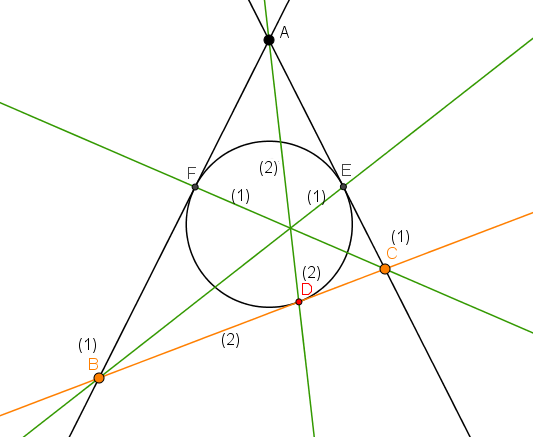
\includegraphics[width=0.7\textwidth]{kepek/kep0.png}
    \end{figure}

    We use the incircle-animation, which comes up very often in problem solving, and which is very useful.

    We start with a general configuration of triangle $ABC$.

    Let's fix $A$, $E$, $F$ and the incircle, and start animating point $D$ with degree 2 on the incircle.

    Since side $BC$ is the polar of $D$ with respect to the incircle, $BC$ has degree 2 too.

    $B$ is the intersection of the fixed side $AB$, and the degree 2 side $BC$. We can use the formula for the intersection point of two lines~\ref{p-ll} to calculate the degree of $B$, that is

    $$\deg (B)= \deg (AB) + \deg (BC) - \# (AB=BC)=0+2-1=1$$

    $(AB=BC)$ happens exactly once, when $D=F$.

    Similarly $C$ also has degree 1.

    To calculate the degree of $EB$, we use the formula for the line through two points~\ref{l-pp}. That is
    $$\deg (EB)= \deg (B) + \deg (E) - \# (B=E)=1+0-0=1$$
    $B$ and $E$ never coincide.

    Similarly $FC$ also has degree 1.

    For the same reason $AD$ has degree $0+2-0=2$.

    By theorem ~\ref{concurrency} the statement that $BE$, $FC$, $AD$ are concurrent, has degree $\deg BE+\deg FC+\deg AD=1+1+2=4$.

    Then it is sufficient to find 5 special cases where the statement is true.

    \begin{enumerate}
        \item $AB=AC$

        Now $ABC$ is isosceles, and the statement is true for every isosceles triangle by symmetry.

        \item $BA=BC$

        Another isosceles case.
        \item $CA=CB$

        And another.
        \item $D=E$

        This is a degenerate case. $C=E=D$ because of the degeneration. Therefore $AD$, $BE$ and $CF$ all go through this point, so they are concurrent.

        \item $D=F$

        The symmetric pair of the previous case.
    \end{enumerate}
    Now we proved that the statement is true for every position of $D$. Therefore it is true for the original position, which was an arbitrary choice, so the statement is true for every triangle $ABC$.
\end{proof}






\section{Locus of a polynomial moving point}




\begin{theorem} [Locus-theorem]\label{locus}
    $H$ is a degree $n$ polynomial moving point. Then the locus of $H$ is a degree $k$ irreducible algebraic curve, where $k\mid n$. For every smooth point $A$ of the curve, $H$ passes through $A$ $\frac{n}{k}$ times (with p-p mul.). For every order $d$ singularity $B$, $H$ passes through $B$ $\frac{n}{k}\cdot d$ times (with p-p mul.)
\end{theorem}
\begin{example}
\hfill \break
    A degree 1 point is always moving on a fixed line, and takes all its positions once. (with p-p mul.)

    A degree 2 point is either moving on a fixed conic, and takes all its positions once, or it is moving on a fixed line, and takes all its positions twice. (with p-p mul.)
\end{example}
\begin{proof}
    The polynomial format of the degree $n$ point $H$ is $(P,Q,R)$.
    There exists a $d$, such that $\binom{d+2}{2} > dn$. The multiset

    $$S=\{P^aQ^bR^c \mid a+b+c=d\}$$

    has $\binom{d+2}{2}$ elements, and all elements are from $\mathbb{C}[t,s]_h^{dn}$, which is a vector space over $\cc$ of dimension $dn$. Therefore the elements of $S$ are linearly dependent. So there exists $a_i\in \cc$ such that not all $a_i$-s are zero, and

    $$\sum a_iP^aQ^bR^c=0$$

    This means that $H$ is always on an algebraic curve $c$ defined homogeneously by $$\sum a_ix^ay^bz^c=0$$



    % Let $P,Q,R\in \cc[t]$ be the univariate forms of the polynomial format of $H$. Then $H(t)=(P(t):Q(t):R(t))$ for every $t\ne \infty$,  $res_t$ denotes resultant in variable $t$.

    % $res_t(xR(t)-P(t),yR(t)-Q(t))$ is an $x$,$y$-variate polynomial, where for every $(x,y)$ satisfying $res_t(xR(t)-P(t),yR(t)-Q(t))=0$ there exists some $t\ne \infty$ for which $xR(t)-P(t)=yR(t)-Q(t)=0$, therefore $x=\frac{P(t)}{R(t)}, y=\frac{Q(t)}{R(t)}$. This means that at every finite $(x,y)$ point of the $res_t(xR(t)-P(t),yR(t)-Q(t))=0$ affine algebraic curve $H$ passes through at least one time.

    % This isn't true for one $(x,y)$, because here we are using a parametric resultant ($x$ and $y$ are the parameters of the polynomials), and the usual resultant uses polynomials with nonzero main coefficient, while this parametric resultant allows this. When only one polynomial has zero main coefficient, the parametric and the usual resultant
    % differ only by a nonzero multiplier, so they are both zero or both nonzero. The error happens when both polynomials have zero main coefficient, but in this case this is true for only one $(x,y)$, which is actually $H$($\infty$), so $H$ goes through this point of the curve also.

    % Now we have an affine algebraic curve $c$, and $H$ goes through every point of $c$. But since $H$ is continuous on the projective plane, it takes the ideal points of the projective extension of $c$ also.

    We can suppose that $c$ is irreducible. That's because $H$ is on at least one of the components $c_i$ infinitely many times. If we substitute $P(t)$, $Q(t)$ and $R(t)$ in $x,y,z$ respectively in the homogenous form of $c_i$, we get a homogeneous bivariate polynomial, which has infinite zeros, therefore it is constant zero. This means that $H$ is always on $c_i$.

    Let $f:c\to \nn$ be the function indicating how many times $H$ passes through a certain point on $c$. (with p-p mul.)

    We want to show that $f$ is constant, except the singularities, where the value is $d$ times bigger, if $d$ is the degree of the singularity.

    In case $c$ is a line, $f(P)=$ number of $H$ passing through a fixed line going through $P$, which is $n$ by the Point-line theorem ~\ref{point-line}, and thus we proved the statement. From now on we suppose $c$ is not a line.

    $f$ is upper-bounded by $n$, because if $H$ is passing through a fixed point $P$ $n+1$ times, the coordinates of $H-P$ are degree $n$ rational functions with $n+1$ zeros, so they are constant zero, and so the 'moving' point is always the same as the fixed point.

    A point $P\in c$ is \textit{problematic} if it's either singularity or $\exists t_0: \  H(t_0)=P$ and $x'(t_0)=0$, where $x(t)$ is the $x$ coordinate-function of $H$ at $t_0$ according to the charts containing $t_0$ and $P$.

    There are only finitely many problematic points, because there are finitely many singularities, and $x'(t)=0$ finitely many times, or always. In the latter case $c$ is a line.

    Lemma 1: $f$ is locally constant in any nonproblematic point.

    Let $P$ be a point on $c$, that is not problematic. Let $t_1, ...,t_m$ be the times when $H(t_i)=P$ ($0 \leq m\leq n$ times at total). $x(t)$ and $y(t)$, are the euclidean coordinates of $H$ according to the charts containing $t_i$ and $P$.

    Since $P$ is a smooth point, and $\frac{\partial F}{\partial y}\ne0$ at $P$ (otherwise $x'(t)=0)$, we can apply holomorphic implicit function theorem, and so we have a neighborhood $N$ in which the curve looks like a holomorphic $y(x)$ graph.

    By holomorphic inverse function theorem, there exists a neighborhood $T$ of $t_i$, where $x(T)$ is a neighborhood of $x(t_i)$, and $x(t)$ is a bijection between $T$ and $x(T)$ ($x'(t)\ne 0$). In addition we can suppose $x(T) \times y(T) \subset N$, and $x(T) \times y(T)$ doesn't contain problematic points.

    \begin{figure}[H]
    \centering
    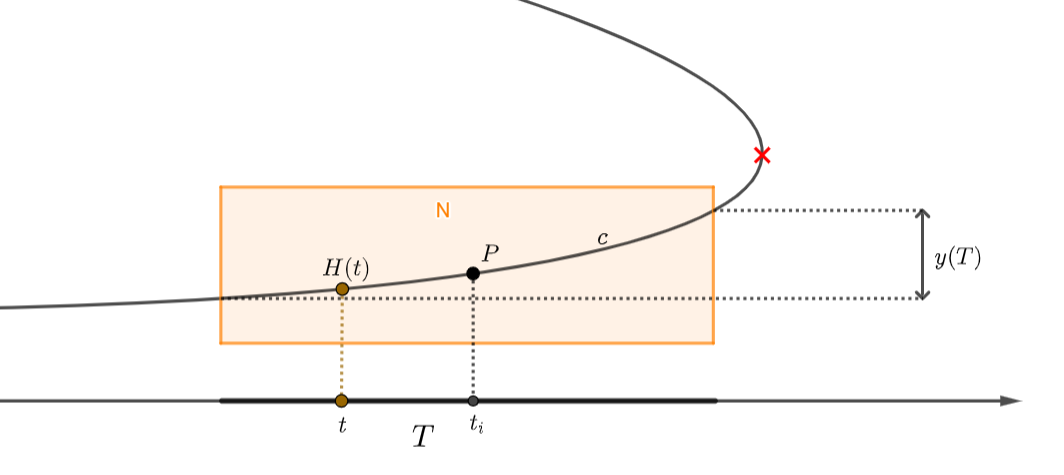
\includegraphics[width=0.8\textwidth]{kepek/locus1.png}
    \end{figure}

    For every $x\in x(T)$, this $x$ value will be held by $H$ for exactly one $t$. In $(x(T) \times y(T)) \cap c$, every $x$ value is held by only one point (it is in $N$), and therefore that one point will be held by $H$ for exactly one $t$. The conclusion is that $H$ goes through every point exactly once in $(x(T) \times y(T)) \cap c$, which is a neighborhood of $H(t_i)$ on $c$. The point-point multiplicity is 1 everywhere, since $x'(t)\ne 0\implies \bigl(x(t),y(t)\bigr)'\ne 0$.

    At every $t_i$, $H$ goes through $P$ with p-p mul. 1 ($x'(t)\ne 0$). So $f(P)=m$. But for every $i$, there is a neighborhood $U_i$ of $P$, where $H$ goes through every point of $U_i$ once within a neighborhood $T_i$ of $t_i$. We can suppose that the $T_i$-s don't intersect. In $U=\bigcap_{i=1}^m U_i$, every point is taken by $H$ exactly $m$ different times within $\bigcup_{i=1}^m T_i$, with mul. 1, so we are left to show that outside of $\bigcup T_i$, $H(t)\ne P$.

    Set $\cc\pp^1\setminus \bigcup T_i$ is compact, so its continuous image via $H$ is also compact, and thus closed. So there exists a $U^*$ neigborhood of $P$, so that $t\notin \bigcup T_i \implies H(t)\notin U^*$.

    Therefore $H$ goes through every point exactly $m$ times in $U\cap U^*$, which means that $f$ is locally constant at $P$.

    With this we proved lemma 1.

    The irreducible $c$ without the problematic points is path-connected, because $c$ without the singular points is path-connected \cite[p.~97]{singpath}, and every smooth point has a neighborhood on $c$, that is homeomorphic to an open set in $\cc$, so omitting finitely many points doesn't affect path-connectedness.

    Let $c'$ be $c$ without the problematic points.

    $f$ is locally constant on $c'$, which is path-connected, so $f$ is constant on all $c'$.

    Lemma 2: A line $l$ is intersecting $c$ at $K$. $l$ is not tangent to $c$ at $K$. Then $$ppmul\big(H(t)=K\big) = plmul\big(H(t)\in l\big)$$

    Using a projective transformation we can suppose that $K$ is the Origin and $l$ is the x-axis. This doesn't change the multiplicities. Line $\lim\Big(\overline{HK}\Big)$ is tangent to $c$, but $l$ is not, so $\lim\Big(\overline{HK}\Big)\ne$ x-axis, or equivalently $\lim \frac{y(t)}{x(t)}\ne 0$, where $x$ and $y$ are the coordinate functions of $H$.
    $$ppmul(H,K)=min\left(\ord(x),\ord(y)\right) = \ord(y)=\ord(\abs{y})=dist(H,\text{x-axis})=plmul(H,l)$$

    \begin{figure}[H]
    \centering
    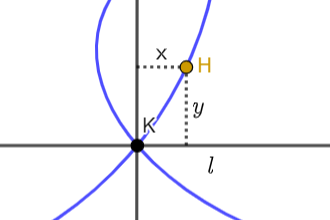
\includegraphics[width=0.3\textwidth]{kepek/locus2.png}
    \end{figure}

    Let $k$ be the degree of $c$.

    Now let $l$ be a line not tangent to $c$, so that no problematic points are on $l$. Then $l$ intersects $c$ at k different non-problematic points $K_i$. The Point-line theorem~\ref{point-line} states that $H$ goes through $l$ a total of $n$ times with point-line mul. By Lemma 2, we know that
    $$n=\sum_t plmul(H,l)=\sum_{i=1}^k \sum_t ppmul(H,K_i)=\sum_{i=1}^k f(K_i)$$
    Since $f$ is constant on $c'$, $f=\frac{n}{k}$. So we proved the theorem for the non-problematic points.

    Let $P$ be a problematic point, which is an order $d$ singularity (we include smooth points too with $d=1$). Let $l$ be a line through $P$, that is not tangent to $c$, and doesn't go through problematic points except $P$. $l$ intersects $c$ at $k-d$ different points not counting $P$. So with similar calculation as above, $f(P)=n-(k-d)\frac{n}{k}=d\cdot\frac{n}{k}$. With this we proved the theorem for problematic points too.

\end{proof}





\subsection{Locus of a polynomial moving line}
\begin{lemma}
    A degree 1 line always has a fixed point around which it rotates, and takes all its positions once. (with l-l mul.)
\end{lemma}
\begin{proof}
    Take a pole-polar transformation, apply the fact that a degree 1 point is moving on a fixed line, and do the inverse of the pole-polar, to get back the original figure, where the degree 1 line always lies on the pole of the fixed line, which is a fixed point. Also the pole-polar equivalent of a point-point multiplicity is a line-line multiplicity.
\end{proof}

\begin{lemma}
    A degree 2 line is either always tangent to a conic, and takes all its positions once, or it has a fixed point around which it rotates, and takes all its positions twice. (with l-l mul.)
\end{lemma}
\begin{proof}
    The pole of the line is a degree 2 point, so there are two cases. First, the pole is moving on a conic, taking all its positions once with p-p mul. This means that the line is always tangent to the dual of this conic, implying the first scenario of the statement. Secondly, the pole is moving on a line taking all its positions twice with p-p mul, implying the second scenario of the statement.
\end{proof}


\section{Mászó-theorem}

While solving a geometry problem, calculating the degree of a line through two points takes a lot of time, because we have to  check all the coincidences of the two points. However when both points move on the same conic, Mászó-theorem gives an explicit degree of the line through them. And also the degree is quite low!

\begin{lemma}
    The degree of a moving point on a fixed conic is always even.
\end{lemma}
\begin{proof}
    The Locus-theorem~\ref{locus} states that if a degree $n$ point moves on a degree $k$ algebraic curve, then $k\mid n$. $k=2$ gives us the proof.
\end{proof}
\begin{theorem}[Mászó-theorem]
Two polynomial points $A$ and $B$ move on the same conic. Then
$$\deg AB = \frac{\deg A+\deg B}{2}$$

\end{theorem}

\begin{proof}

    $\deg A=a$, $ \deg B =b$.
    Let $P$ be a fixed point on the conic $\mathcal{C}$, and $l$ a line not passing through $P$. According to the Locus-theorem~\ref{locus}, since $A$ moves on $\mathcal{C}$, it passes through $P$ exactly $\frac{a}{2}$ times (with p-p mul.) This means that the line $AP$ has degree $0+a -\frac{a}{2}=\frac{a}{2}$. Let $A'=AP\cap l$, $B'$ similarly. $\deg A'=0+\frac{a}{2}-0=\frac{a}{2}$. Similarly $\deg B'=\frac{b}{2}$. $A'$ and $B'$ are both moving on $l$, so applying Lemma ~\ref{degab} they coincide exactly $\frac{a}{2}+\frac{b}{2}$ times (with p-p multiplicity).

    \begin{figure}[H]
    \centering
    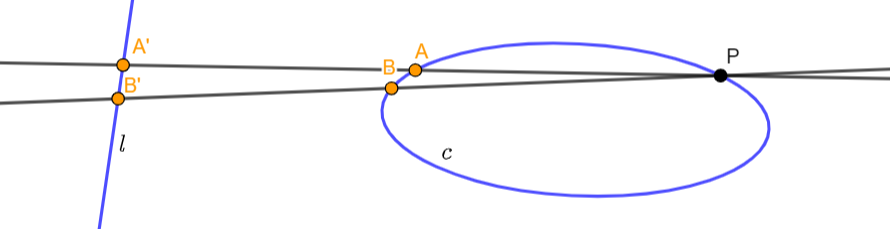
\includegraphics[width=1\textwidth]{kepek/maszoth.png}
    \end{figure}

    Let $C$ be a degree $2$ moving point on the conic. We construct $C'$ similarly as before, so $\deg C'=1$.
    $C'$ as a function of time is a biholomorphism between $l$ and $\cc\pp^1$, because the Locus-theorem states that $C'(t)$ goes through at every point of $l$ exactly once with nonzero derivative. We can apply the Inverse function theorem to get that $C'^{-1}$ exists, and is holomorphic. For the same reason, $C$ as a function of time is a biholomorphism between $\mathcal{C}$ and $\cc\pp^1$.
    The $\phi: C(t)\mapsto C'(t)$ mapping is a biholomorphism, because $\phi=C'\circ C^{-1}$.

    We can now apply the p-p multiplicity lemma ~\ref{ppmul}, to conclude that the p-p mul. of $A$ and $B$ is the same as of $A'$ and $B'$.

    This means that $A$ and $B$ coincide exactly the same number of times as $A'$ and $B'$ do, which is $\frac{a+b}{2}$.

    We know that $\deg AB=a+b-\#(A=B)=a+b-\frac{a+b}{2}=\frac{a+b}{2}$.

\end{proof}

We use the next theorem in a geometry problem when we construct the second intersection point of a circle and a line, such that the first intersection point is already given.

\begin{theorem} [Inverse of Mászó-theorem]

    Let $\mathcal{C}$ be a fixed conic, $A$ a polynomial moving point on it, and $l$ a polynomial line always going through $A$. The second intersection of $\mathcal{C}$ and $l$ is $B$. Then $B$ is polynomial, and its degree satisfies

    $$\deg l = \frac{\deg A+\deg B}{2}$$

\end{theorem}
\begin{proof}

    With a projective transformation we can send any conic into a circle, so we can suppose $\mathcal{C}$ is a circle with center $O$. $l$ has a polynomial ideal point (intersection with the ideal line, which is fixed). A 90° rotation sends this ideal point into the perpendicular direction's ideal point, so connecting this with $O$ gives us a polynomial line, which is the perpendicular bisector of $A$ and $B$. A polynomial point's reflection across a polynomial line is also polynomial, and therefore $B$ is polynomial.

    We can now use Mászó-theorem to conclude that indeed $$\deg l = \frac{\deg A+\deg B}{2}$$
\end{proof}


\begin{theorem}
    Let $A$ and $B$ be two polynomial moving points on a fixed conic. Then the degree of the statement "$A$=$B$" is $\frac{\deg A+ \deg B}{2}$ (with point-point multiplicity).
\end{theorem}
\begin{proof}
    Mászó-theorem:
    $\deg AB=\frac{\deg A+\deg B}{2}$

    L-pp theorem:
    $\deg AB=\deg A+\deg B-\#(A=B)$ $\implies \#(A=B)=\frac{\deg A+\deg B}{2}$

    We use p-p multiplicity to calculate $\#(A=B)$.
\end{proof}

\section{Moving conics}
\subsection{Basic statements}
When the problem contains several circles, it is usually impossible to find an animation that fixes all circles. So we need to deal with moving circles too. We have already defined moving conics, now we look at all the relevant construction steps and statements about them.

\begin{theorem}
    Let $P$ be a polynomial moving point, and let $c$ be a polynomial moving conic. Then the degree of the statement "$P$ is on $c$" is
    $$2\deg P+ \deg c$$
\end{theorem}
\begin{proof}
    The point $P=(x:y:z)$ is on the conic $(A:B:C:D:E:F)$ iff
    $$Ax^2+Bxy+Cy^2+Dxz+Eyz+Fz^2=0$$
    This is a degree $2\deg P+ \deg c$ polynomial of time. Therefore it has exactly $2\deg P+ \deg c$ roots or it is constant zero.
\end{proof}

\begin{theorem}\label{6onconic}
    Let $P_i$ $(i=1,\ldots ,6)$ be 6 polynomial moving points.
    Then the degree of the statement "The $P_i$ are on a conic" is
    $$2\cdot \sum_{i=1}^6 \deg P_i$$
\end{theorem}
\begin{proof}
The 6 points are on a conic if and only if
   $$ \det
\begin{pmatrix}
x_1^2 & x_1 y_1 & y_1^2 & x_1 z_1 & y_1 z_1 & z_1^2 \\[4pt]
x_2^2 & x_2 y_2 & y_2^2 & x_2 z_2 & y_2 z_2 & z_2^2 \\[4pt]
x_3^2 & x_3 y_3 & y_3^2 & x_3 z_3 & y_3 z_3 & z_3^2 \\[4pt]
x_4^2 & x_4 y_4 & y_4^2 & x_4 z_4 & y_4 z_4 & z_4^2 \\[4pt]
x_5^2 & x_5 y_5 & y_5^2 & x_5 z_5 & y_5 z_5 & z_5^2 \\[4pt]
x_6^2 & x_6 y_6 & y_6^2 & x_6 z_6 & y_6 z_6 & z_6^2
\end{pmatrix}
= 0$$
This determinant is a degree $2\cdot \sum_{i=1}^6 \deg P_i$ polynomial of time.
\end{proof}

\subsection{The symmetric matrix of a conic}

A $c=\{Ax^2+Bxy+Cy^2+Dxz+Eyz+Fz^2=0\}$ conic can be represented with a symmetric matrix $M$, for which $x$ is on the conic if and only if $x^TMx=0$.
$$M=\begin{pmatrix}
A & \tfrac{B}{2} & \tfrac{D}{2} \\
\tfrac{B}{2} & C & \tfrac{E}{2} \\
\tfrac{D}{2} & \tfrac{E}{2} & F
\end{pmatrix}
$$
The elements of $M$ are degree $\deg c$ polynomials of time with no common root.

\begin{theorem}
    Let $c$ be a polynomial moving conic. Then the image of $c$ with respect to a fixed projective transformation is also a polynomial moving conic with degree $\deg c$.
\end{theorem}
\begin{proof}
    The conic $c$ has symmetric matrix $M$. Then the equation of $c$ is $x^TMx=0$. The projective transformation has matrix $A$. So a point $x$ is on the image of $c$ if and only if the preimage of $x$ is on $c$. This can be expressed as $(A^{-1}x)^TM(A^{-1}x)=0$ or $x^T(A^{-1})^TMA^{-1}x=0$. $A$ is constant, $M$ has coordinates of degree $\deg c$, and so has $(A^{-1})^TMA^{-1}$. Since both $(A^{-1})^T$ and $A^{-1}$ is invertible, $(A^{-1})^TMA^{-1}$ cannot be the zero matrix. Therefore the symmetric matrix $(A^{-1})^TMA^{-1}$ also corresponds to a degree $\deg c$ polynomial moving conic.
\end{proof}

The rank of $M$ determines how the conic looks:

\begin{itemize}
    \item $\mathrm{rk}M=3$: The conic is nondegenerate
    \item $\mathrm{rk}M=2$: The conic splits into two different lines
    \item $\mathrm{rk}M=1$: The conic is a single line counted twice
\end{itemize}


The \textit{adjugate matrix} $\mathrm{adj}(M)$ of $M$ consists of the $2\times 2$ subdeterminants of $M$ with a sign, these are what we calculate when determining the inverse of $M$. Thus $\mathrm{adj}(M)$=$\det M \cdot M^{-1}$ when $\det M\ne 0$.

For any two matrices $A$ and $B$, $\mathrm{adj}(AB)=\mathrm{adj}(B)\mathrm{adj}(A)$, and also $\mathrm{adj}(M^T)=\mathrm{adj}(M)^T$

While using homogeneous coordinates, taking $\mathrm{adj}(M)$ instead of $M^{-1}$ doesn't change the result, because they differ only by a scaling factor. However, $\mathrm{adj}(M)$ is always defined, even if $\det M=0$. Furthermore it is polynomial in the elements of $M$.

With the use of $\mathrm{adj}(M)$ we can prove the following theorem.
\begin{theorem}
    Let $l$ be a polynomial moving line, and let $c$ be a polynomial moving conic. Then the degree of the statement "$l$ is tangent to $c$" is

    $$2\deg l+ 2\deg c$$
\end{theorem}
\begin{remark}

    Here "$l$ is tangent to $c$" means:
\begin{itemize}
    \item $\mathrm{rk}M=3$: The conic is nondegenerate, and $l$ is tangent to it
    \item $\mathrm{rk}M=2$: The conic splits into two different lines, and $l$ goes through the intersection point of the two lines
    \item $\mathrm{rk}M=1$: The conic is a single line counted twice, in this case every line $l$ is tangent to it.
\end{itemize}
\end{remark}
\begin{proof}
    The statement "$l$ is tangent to $c$" is equivalent to $l^T\mathrm{adj}(M) l=0$. To prove this, we look at the three cases:

    \begin{itemize}
    \item $\mathrm{rk}M=3$: The polar $l$ of $P$ w.r.t. $c$ is $l=Mp$, and thus the pole $P$ of $l$ w.r.t. is $p=M^{-1}l$ with homogeneous coordinates. $l$ is tangent to $c$ iff its pole $P$ is on $c$. So this is equivalent to $(M^{-1}l)^TM(M^{-1}l)=0$. Simplifying, we get $l^TM^{-1}l=0$, multiplying by $\det M\ne0$ we get $l^T\mathrm{adj}(M) l=0$.
    \item $\mathrm{rk}M=2$: The conic splits into two different lines. A projective transformation with matrix $A$ takes $c$ to the union the $x$-axis and the $y$-axis. This projective transformation sends any line $l$ to $(A^{-1})^Tl$, and any conic with symmetric matrix $M$ to a conic with symmetric matrix with $(A^{-1})^TMA^{-1}$, as we have seen in the previous theorem. Furthermore the condition $l^T\mathrm{adj}(M) l=0$ is invariant under the transformation. That's because
    $$((A^{-1})^Tl)^T\mathrm{adj}((A^{-1})^TMA^{-1})((A^{-1})^Tl)=0\iff l^T\mathrm{adj}(M) l=0$$
    The geometric condition for tangency is also preserved under the projective transformation.
    So we need to check only for the conic $\{xy=0\}$ if the statement is true. The $\{xy=0\}$ has symmetric and adjugate matrices
    $$M =
\begin{bmatrix}
0 & \tfrac{1}{2} & 0\\[4pt]
\tfrac{1}{2} & 0 & 0\\[4pt]
0 & 0 & 0
\end{bmatrix}
\quad
\operatorname{adj}(M) =
\begin{bmatrix}
0 & 0 & 0\\[4pt]
0 & 0 & 0\\[4pt]
0 & 0 & -\tfrac{1}{4}
\end{bmatrix}$$

Now
$l^T\mathrm{adj}(M) l=0 \iff$ the last coordinate of $l$ is zero $\iff$ $(0:0:1)$ is on $l$ $\iff$ $l$ goes through the origin, which is the intersection of the $x$-axis and the $y$-axis, and that's exactly the geometric condition that we wanted to prove.


    \item $\mathrm{rk}M=1$: The conic is a single line counted twice, and we want to prove that for every line $l$, $l^T\mathrm{adj}(M) l=0$. But since $\mathrm{rk}M=1$, all $2\times 2$ subdeterminants of $M$ are zero, thus $\mathrm{adj}(M)=0$.
\end{itemize}

    So $l^T\mathrm{adj}(M) l=0$ is the polynomial expression for "$l$ is tangent to $c$". All elements of $\mathrm{adj}(M)$ are the 2x2 subdeterminants of $M$ with a sign. So all elements have degree $2\deg c$, therefore by expanding the matrix multiplication of $l^T\mathrm{adj}(M) l=0$, we get a degree $2\deg l+ 2\deg c$ polynomial of time.
\end{proof}


\subsection{Pole-polar with respect to moving conic}





\begin{theorem}
    Let $P$ be a polynomial moving point, and let $c$ be a polynomial moving conic. Then the degree of the polar $l$ of $P$ with respect to $c$ is at most
    $$\deg l\le\deg P +\deg c - \#(\text{"$c$ splits into 2 lines, and $P$ is the intersection" or}$$
    $$\text{"$c$ is a line, and $P$ is on this line"})$$
\end{theorem}
\begin{proof}
    The symmetric matrix of $c$ is $M$. Then the polar $l$ is determined by $l=Mp$ using homogeneous coordinates. So $l$ has coordinates of degree $\deg c+\deg P$, but there may be common roots, so we have to subtract the number of the events "$Mp=0$" to get the degree of $l$. We have 3 cases again:
    \begin{itemize}
    \item $\mathrm{rk}M=3$: The conic is nondegenerate, and since $p\ne 0$, $Mp=0$ is not possible.
    \item $\mathrm{rk}M=2$: The conic splits into two different lines. We want to prove that $Mp=0$ is equivalent to "$P$ is the intersection point of the two lines". As previously, we take the projective transformation with invertible matrix $A$ which takes $c$ to $\{xy=0\}$. This preserves the condition $Mp=0$, because
    $$((A^{-1})^TMA^{-1})(Ap)=0 \iff Mp=0$$

    For $\{xy=0\}$,
    $$M=\begin{bmatrix}
0 & \tfrac{1}{2} & 0\\[4pt]
\tfrac{1}{2} & 0 & 0\\[4pt]
0 & 0 & 0
\end{bmatrix}$$
therefore $Mp=0 \iff$ the first two coordinates of $p$ is zero $\iff$ $P=$ origin, which is the intersection point of the $x$-axis and the $y$-axis.
    \item $\mathrm{rk}M=1$: The conic is a single line counted twice. We want to prove that $Mp=0$ is equivalent to "$P$ is on $c$". We take the projective transformation sending $c$ to the line $\{x^2=0\}$. The symmetric matrix of $\{x^2=0\}$ is
    $$M=\begin{bmatrix}
    1 & 0 & 0\\[4pt]
    0 & 0 & 0\\[4pt]
    0 & 0 & 0
    \end{bmatrix}$$
    $Mp=0 \iff$ the $x$ coordinate of $P$ is zero $\iff$ $P$ is on $c$
\end{itemize}
\end{proof}



% \begin{lemma}
%     Let $M \in \cc^{3x3}$ be a polynomial matrix, with $\mathrm{rk}(M)$ not constant 1, and $\mathrm{adj}(M)$ its adjugate matrix. Then $\mathrm{adj}(M)$ is polynomial, and

%     $$\deg (\mathrm{adj}(M))=2 \deg M - \#(\mathrm{rk}(M)=1)$$
% \end{lemma}
% \begin{proof}
%     All elements of $\mathrm{adj}(M)$ are the 2x2 minors of $M$ with a sign, which is not important here. So all elements are of degree $2\deg M$, or they are constant zero. $\mathrm{rk}(M)$ is not constant 1, so $\mathrm{adj}(M)$ is not constant zero. We have to distribute the number times when $\mathrm{adj}(M)=0$, this is equivalent to $\mathrm{rk}(M)=1$
% \end{proof}


\begin{theorem}
    Let $l$ be a polynomial moving line, and let $c$ be a polynomial moving conic. Then the degree of the pole $P$ of $l$ with respect to $c$ is at most
    $$\deg P\le\deg l +2\deg c - \#(\text{"$c$ splits into 2 lines, and $l$ goes through the intersection" or "$c$ is a line"})$$
\end{theorem}
\begin{proof}
    The pole $p$ is derived by $p=M^{-1} l$ if $\det M\ne 0$. This is a rational function, and but we can write this equivalently as $p=\mathrm{adj}(M) l$, which is polynomial. So $p$ has coordinates of degree $\deg l +2\deg c$, and from this we have to subtract the number of times when $\mathrm{adj}(M) l=0$. According to the tried and tested method we can take the 3 cases:
    \begin{itemize}
    \item $\mathrm{rk}M=3$: $M$ is invertible, therefore $\mathrm{adj}(M)$ is invertible too. Since $l\ne 0$, $\mathrm{adj}(M)l=0$ is not possible.
    \item $\mathrm{rk}M=2$: The conic splits into two different lines. We want to prove that $\mathrm{adj}(M)l=0$ is equivalent to "$l$ goes through the intersection point of the two lines". As usual, we take the projective transformation with invertible matrix $A$, which takes $c$ to $\{xy=0\}$. This preserves the condition $\mathrm{adj}(M)l=0$, because
    $$\mathrm{adj}((A^{-1})^TMA^{-1})((A^{-1})^Tl)=0 \iff \mathrm{adj}(M)l=0$$

    For $\{xy=0\}$,
    $$\operatorname{adj}(M) =
    \begin{bmatrix}
    0 & 0 & 0\\[4pt]
    0 & 0 & 0\\[4pt]
    0 & 0 & -\tfrac{1}{4}
    \end{bmatrix}$$
therefore $\mathrm{adj}(M)l=0\iff$ the last coordinate of $l$ is zero $\iff$ $(0:0:1)$ is on $l$ $\iff$ $l$ goes through the origin, which is the intersection of the $x$-axis and the $y$-axis.
    \item $\mathrm{rk}M=1$: The conic is a single line counted twice, and we want to prove that for every line $l$, $\mathrm{adj}(M) l=0$. But we know that $\mathrm{adj}(M)=0$, so the statement follows.
\end{itemize}
\end{proof}



\begin{corollary}
    A degree 1 moving conic always goes through some fixed points and is tangent to some fixed lines which can be
    \begin{itemize}
        \item 4 points
        \item 3 points and a line through one of them
        \item 2 points and 2 lines, one through each point
        \item 2 points, and a line through one of them
        \item 1 point, and a line through it.
    \end{itemize}
\end{corollary}
\begin{proof}
    Take two positions of the moving conic (when they are nondegenerate), $c_1$ and $c_2$. They intersect in 4 points, with multiplicity. So there are 5 cases:
    \begin{itemize}
        \item $c_1$ and $c_2$ intersect in 4 different points. Then we know that a fixed point $P$ is on the moving conic $c$ exactly $\deg P+\deg c=0+1=1$ times, or $P$ is always on $c$. Here, we already know two positions of $c$, where $P$ is on $c$, these are $c_1$ and $c_2$. So $P$ is necessarily always on $c$. This is true for all 4 intersection points, so $c$ is always going through these points.
        \item $c_1$ and $c_2$ intersect in 3 different points, with multiplicity 1, 1, and 2. Just like in the previous case, we know that $c$ is going through all 3 points. Let $P$ be the intersection point with multiplicity 2. Let $l$ be the common tangent of $c_1$ and $c_2$ at this point. The polar of $P$ with respect of $c$ is the tangent at $P$ to $c$. This has degree at most $\deg P + \deg c=0+1=1$. If a degree 1 line is taking one of its positions twice, it must be constant. This is the case here too, because $l$ is the tangent in $P$ to $c_1$ and $c_2$ also. So $c$ is always tangent to the fixed line $l$.
        \item $c_1$ and $c_2$ intersect in 2 different points, with multiplicity 2 and 2. By the same reason as before we get that $c$ always goes through the 2 points, and it is always tangent to 2 lines through the 2 points.
        \item $c_1$ and $c_2$ intersect in 2 different points, with multiplicity 3 and 1. Again, $c$ always goes through the 2 points, and it is always tangent to the common tangent line at the multiplicity 3 point.
        \item $c_1$ and $c_2$ intersect in 1 point, with multiplicity 4. Then $c$ always goes through this point, and it is always tangent to the common tangent line at this point.
    \end{itemize}
\end{proof}

\subsection{Constructing moving conics}

\begin{theorem}\label{conicthr5}
    Let $P_1$, $P_2$, $P_3$, $P_4$ and $P_5$ be five polynomial moving points. Then the conic $c$ always going through them is polynomial, and its degree is at most
    $$\deg c\le 2\cdot\sum_{i=1}^5\deg P_i-\#(\text{"any two points are the same" or "any 4 points are collinear"})$$
\end{theorem}
\begin{proof}
    In $\cc\pp^5$ $(A:B:C:D:E:F)$ corresponds to the conic $c$. Let $P_i=(x_i:y_i:z_i)$
    For every $i=1,\ldots ,5$ $$Ax_i^2+Bx_iy_i+Cy_i^2+Dx_iz_i+Ey_iz_i+Fz_i^2=0$$
    So $(A,B,C,D,E,F)$ is orthogonal to all five $(x_i^2, x_iy_i, y_i^2, x_iz_i, y_iz_i, z_i^2)$ vectors in $\cc^6$.
    We can calculate $(A,B,C,D,E,F)$ analogously to the cross product in 3 dimension:
    $A$, $B$, $C$, $D$, $E$ and $F$ must be the corresponding $5\times5$ signed subdeterminants of the matrix

    $$M=
    \begin{bmatrix}
    x_1^2 & x_1 y_1 & y_1^2 & x_1 z_1 & y_1 z_1 & z_1^2 \\[4pt]
    x_2^2 & x_2 y_2 & y_2^2 & x_2 z_2 & y_2 z_2 & z_2^2 \\[4pt]
    x_3^2 & x_3 y_3 & y_3^2 & x_3 z_3 & y_3 z_3 & z_3^2 \\[4pt]
    x_4^2 & x_4 y_4 & y_4^2 & x_4 z_4 & y_4 z_4 & z_4^2 \\[4pt]
    x_5^2 & x_5 y_5 & y_5^2 & x_5 z_5 & y_5 z_5 & z_5^2
    \end{bmatrix}$$

    Thus $A$, $B$, $C$, $D$, $E$ and $F$ are degree $2\cdot\sum_{i=1}^5\deg P_i$ polynomials of time.
    Now we have to subtract the number of times when $(A,B,C,D,E,F)=(0,0,0,0,0,0)$. This is equivalent to $\mathrm{rk}M\le 4$.

    If any two of the five $P_i$-s are the same, then obviously two rows of $M$ are the same ensuring $\mathrm{rk}M\le 4$.

    The map $v:\cc^3\to \cc^6\quad (x,y,z)\mapsto (x^2,xy,y^2,xz,yz,z^2)$ has the following property:
    every $\varphi$ linear transformation on $\cc^3$ induces a $\Phi$ linear transformation on $\cc^6$ such that $$v(\varphi(p))=\Phi(v(p))$$

    Any projective transformation on $\cc\pp^2$ acts linearly on $(x_i,y_i,z_i)\in \cc^3$, which therefore makes all five $(x_i^2, x_iy_i, y_i^2, x_iz_i, y_iz_i, z_i^2)$ vectors change by a linear transformation. And this of course doesn't affect the condition
    $\mathrm{rk}M\le 4$.

    If 4 points are on the same line (assume the first 4), we can send that line to $\{z=0\}$, making the $z$ coordinate in $P_1$, $P_2$, $P_3$ and $P_4$ zero. This makes the $xz$, $yz$ and $z^2$ columns in $M$ pairwise linearly dependent, so in any 5x5 subdeterminant we can find 2 linearly dependent columns, making $\mathrm{rk}M\le 4$.

    Now we are only left to show that when no 2 points are the same, and no 4 points are collinear, then $\mathrm{rk}M= 5$.

    In such case we can find 4 points out of which no 3 are collinear. We can send these to the 4 base points $(1:0:0)$, $(0:1:0)$, $(0:0:1)$ and $(1:1:1)$ with a projective transformation, and with this
    $$M=
    \begin{bmatrix}
    1 & 0 & 0 & 0 & 0 & 0 \\[4pt]
    0 & 0 & 1 & 0 & 0 & 0 \\[4pt]
    0 & 0 & 0 & 0 & 0 & 1 \\[4pt]
    1 & 1 & 1 & 1 & 1 & 1 \\[4pt]
    x_5^2 & x_5 y_5 & y_5^2 & x_5 z_5 & y_5 z_5 & z_5^2
    \end{bmatrix}$$

    We know that $P_5$ is not equal to any of the 4 base points, therefore with a little casework we get that 2 out of the numbers $x_5 y_5$, $x_5 z_5$ and $y_5 z_5$ are different. We pick the 2 columns corresponding to these numbers together with columns 1, 3 and 6. It is easy to check that the 5x5 submatrix made by these columns has nonzero determinant, ensuring $\mathrm{rk}M= 5$
\end{proof}

\subsection{Intersection}

\begin{theorem}
    Let $l$ be a polynomial moving line and let $c$ be a polynomial moving conic. Then their 2 intersection points $A,B$ form a square root point pair with degree
    $$2\deg (A,B)= \deg c + 2\deg l-\#(\text{$c$ contains $l$ as a component})$$
\end{theorem}
\begin{remark}
    If one of $A$, $B$ is polynomial, then the other is so, and the formula with polynomial degrees is
    $$\deg A+\deg B= \deg c + 2\deg l-\#(\text{$c$ contains $l$ as a component})$$
\end{remark}
\begin{proof}

[unfinished]

    Let $f$ be a fixed line that never coincides with $l$.

    If $A$ and $B$ are polynomial, then we know that the statement "$A$ is on $f$" has degree $\deg A$, and the statement "$B$ is on $f$" has degree $\deg B$.

    We know that "$A$ is on $f$" or "$B$ is on $f$" or "$c$ contains $l$ as a component" is equivalent to "$f$, $l$ and $c$ have a common intersection point", which is equivalent to "$f\cap l$ is on $c$".

    Let $f\cap l$ be $P$. Then $\deg P=\deg f+\deg l-\#(f=l)=0+\deg l-0=\deg l$.

    The statement "$P$ is on $c$" has degree $2\deg P +\deg c$.

    Comparing the beginning and the end we get
    $$\deg A+\deg B+\#(\text{$c$ contains $l$ as a component})\le2\deg P +\deg c=2\deg l +\deg c$$
\end{proof}

\begin{theorem}
    Let $c_1$ and $c_2$ be two polynomial moving circles. Then their 2 intersection points $A,B$ form a square root point pair with degree
    $$2\deg (A,B)=2\deg c_1 + 2\deg c_2-\#(\text{$c_1$ and $c_2$ have a common component})$$
\end{theorem}
\begin{remark}
    If one of $A$, $B$ is polynomial, then the other is so, and the formula with polynomial degrees is
    $$\deg A+\deg B= 2\deg c_1 + 2\deg c_2-\#(\text{$c_1$ and $c_2$ have a common component})$$
\end{remark}
\begin{remark}
    The multiplicity of $\#(\text{$c_1$ and $c_2$ have a common component})$ at $t_0$ is at least 2 if $c_1=c_2$ at $t_0$.
\end{remark}
\begin{proof}

    [unfinished]
\end{proof}

\begin{theorem}
    Let $c_1$ and $c_2$ be two polynomial moving conics. Then their 4 intersection points $A,B,C,D$ are not necessarily polynomial, but if they are, then
    $$\deg A+\deg B+\deg C+\deg D\le2\deg c_1 + 2\deg c_2-\#(\text{$c_1$ and $c_2$ have a common component})$$
\end{theorem}
\begin{proof}

    [unfinished]
\end{proof}

\section{Moving circles}

\subsection{Constructing circles}

\begin{definition}
    We call the points with homogeneous coordinates $(1:i:0)$ and $(1:-i:0)$ the two \textit{circle points}, denoted by $\alpha_i$ and $\alpha_{-i}$
\end{definition}

These are the ideal points of the lines with slope $i$ and $-i$.

\begin{lemma}
    Every circle passes through the circle points.
\end{lemma}
\begin{proof}
    The homogeneous equation of a circle with radius $r$ and center $(v,w)$ is
    $$(x-vz)^2+(y-wz)^2-r^2z^2=0$$
    Substituting $(1:i:0)$ and $(1:-i:0)$ returns zero.
\end{proof}

So a circle is a conic that goes through the two circle points $\alpha_i$ and $\alpha_{-i}$. The degree of a moving circle is its degree as a conic.

Previously we calculated the degree of the conic through 5 points ~\ref{conicthr5}. If we apply this with 2 points being constant $\alpha_i$ and $\alpha_{-i}$ we get the degree of the circle through 3 points:

\begin{theorem}
    Let $P_1$, $P_2$ and $P_3$ be three polynomial moving points. Then their circumcircle $c$ is polynomial, and its degree is at most
    $$\deg c\le 2(\deg P_1+\deg P_2+\deg P_3)-\#(\text{"any two points are the same" or "any point is one of the circle points"}$$
    $$\text{or "any 2 points are on the ideal line" or "all 3 points are collinear on a line with slope $i$ or $-i$"})$$
\end{theorem}

With the same observation we get the following theorem from a previous one ~\ref{6onconic}:
\begin{theorem}
    Let $P_i$ $(i=1,2,3,4)$ be 4 polynomial moving points.
    Then the degree of the statement "The $P_i$ are on a circle" is
    $$2\cdot \sum_{i=1}^4 \deg P_i$$
\end{theorem}

We can characterise circles in another way via its equation. We know that the equation of the circle is $x^2+y^2+Dx+Ey+F=0$. With homogeneous coordinates this yields that a conic $(A:B:C:D:E:F)$ is a circle iff $A=C$ and $B=0$, in other words it can be written as $(A:0:A:D:E:F)$.

\begin{theorem}
    Let $c$ be a polynomial moving circle. Then its center $O$ is a polynomial moving point with degree at most

    $$\deg O\le\deg c-\#(c=\text{ideal line counted twice})$$
\end{theorem}
\begin{proof}
    The equation of the circle $(A:0:A:D:E:F)$ can be written as
    $$\left(\frac{x}{z}+\frac{D}{2A}\right)^2+\left(\frac{y}{z}+\frac{E}{2A}\right)^2+\frac{F}{A}-\frac{D^2}{4A^2}-\frac{E^2}{4A^2}=0$$
    So $O$ is
    $$\left(-\frac{D}{2A},-\frac{E}{2A}\right)=(D:E:-2A)$$
    This has coordinates of degree $\deg c$, and we have to subtract the number of times when $(D,E,-2A)=(0,0,0)$. This is equivalent to $c=(0:0:0:0:0:F)$, which is the ideal line counted twice.
\end{proof}


\begin{theorem}
    Let $O$ and $P$ be two polynomial moving points. The circle $c$ with center $O$ that goes through $P$ is polynomial, and has degree at most
    $$\deg c\le \deg O+2\deg P-\#(\text{"$P$ is one of the circle points" or "$P$ and $O$ are both ideal points"})$$
\end{theorem}
\begin{proof}
    Let $O=(u:v:w)$, $P=(x:y:z)$ and $c=(A:0:A:D:E:F)$. Then by the previous reasons $(D:E:-2A)=(u:v:w)$, and
    $$\frac{F}{A}=\frac{D^2}{4A^2}+\frac{E^2}{4A^2}-\left(\frac{x}{z}+\frac{D}{2A}\right)^2-\left(\frac{y}{z}+\frac{E}{2A}\right)^2=\left(\frac{u}{w}\right)^2+\left(\frac{v}{w}\right)^2-\left(\frac{x}{z}-\frac{u}{w}\right)^2-\left(\frac{y}{z}-\frac{v}{w}\right)^2$$

Multiplying by the common denominator

$$(A:0:A:D:E:F)=(w^2z^2:0:w^2z^2:-2uwz^2:-2vwz^2:u^2z^2+v^2z^2-(wx-uz)^2-(wy-vz)^2)\overset{\text{/$w$}}{=}$$
$$=(wz^2:0:wz^2:-2uz^2:-2vz^2:-wx^2+2xuz-wy^2+2yvz)$$

All the coordinates are degree $\deg O+2\deg P$. From this we have to subtract the number of times when $(A,0,A,D,E,F)=0$. Since the first component is $wz^2$, this case can only happen when either $w=0$ or $z=0$. When $z=0$, the first 5 coordinates are zero, and the last one is $-(wx)^2-(wy)^2$. This zero iff $w=0$ or $x^2+y^2=0$, in other words $P=(x:y:z)$ is one of the circle points. When $w=0$, $u$ and $v$ can't be zero at the same, otherwise $O=(0:0:0)$, which is impossible. Then since $-2uz^2$ and $-2vz^2$ are both zero, $z$ must be zero.
The conclusion is that $(A,0,A,D,E,F)=0$ iff $P$ is one of the circle points or $P$ and $O$ are both ideal points.
\end{proof}

\begin{theorem}
    Let $O$ be a polynomial moving point, and $r^2$ be a polynomial quantity. Then the circle $c$ with center $O$ and radius $r$ has degree at most
    $$\deg c\le \deg r^2+2\deg O-\#("\text{$O$ is an ideal point and $r^2=\infty$" or "$O$ is one of the circle points"})$$
\end{theorem}
\begin{proof}
    Let $O=(u:v:w)$ and $r^2=\frac{p}{q}$

    Then the equation of $c$ can be written as
    $$\left(\frac{x}{z}-\frac{u}{w}\right)^2+\left(\frac{y}{z}-\frac{v}{w}\right)^2-\frac{p}{q}=0$$
    Multiplying with the common denominator:
    $$q(wx-uz)^2+q(wy-vz)^2-pw^2z^2=0$$
    After expanding parentheses, $c$ is
    $$(qw^2:0:qw^2:-2qwu:-2qwv:q(u^2+v^2)-pw^2)$$
    All coordinates has degree $\deg r^2+2\deg O$. From this we have to subtract the number of times when all coordinates are zero. Looking at the first coordinate, this can only happen when either $q=0$ or $w=0$.

    If $w=0$, then the first 5 coordinates are automatically 0, and the last is 0 iff $q=0$ or $u^2+v^2=0$, that is $r^2=\infty$ or $O$ is one of the circle points.

    If $q=0$, then the first 5 coordinates are automatically 0 again, and the last is 0 iff $pw^2=0$, that is $p=0$ or $w=0$. The former is not possible, since $p$ and $q$ does not have a common root, and the latter was already done previously.
\end{proof}

\begin{theorem}
    Let $A$ and $B$ be two polynomial moving points. Then their Thales circle $c$ is polynomial, and its degree is at most
    $$\deg c\le \deg A+\deg B-\#(\text{$A$ and $B$ are ideal points of perpendicular direction})$$
\end{theorem}
\begin{proof}
    Let $A=(a_1,a_2)$ and $B=(b_1,b_2)$ be two finite points, then their Thales circle has equation
    $$\left(x - \frac{a_1 + b_1}{2}\right)^2 + \left(y - \frac{a_2 + b_2}{2}\right)^2
- \frac{(b_1 - a_1)^2 + (b_2 - a_2)^2}{4}=0$$
By expanding the parentheses we get
$$x^2 + y^2 - (a_1 + b_1)x - (a_2 + b_2)y + (a_1 b_1 + a_2 b_2) = 0$$
Homogenising:
$$a_3b_3x^2 + a_3b_3y^2 - (a_1b_3 + b_1a_3)xz - (a_2b_3 + b_2a_3)yz + (a_1 b_1 + a_2 b_2)z^2 = 0$$
$$c=(a_3b_3:0:a_3b_3:-(a_1b_3 + b_1a_3):-(a_2b_3 + b_2a_3):a_1 b_1 + a_2 b_2)$$

These are degree $\deg A+\deg B$ polynomials, so we have to subtract the number of times when $c=(0:0:0:0:0:0)$. This is only possible when $a_3=0$ or $b_3=0$ (1. component). When $a_3=0$, $a_1b_3=a_2b_3=0$ (4. and 5. component), and since $(a_1,a_2,a_3)\ne (0:0:0)$ $b_3$ must be zero too. So both $A$ and $B$ are ideal points, and the last component ensures that they their slopes' product is $-1$, therefore they are in perpendicular direction
\end{proof}


\subsection{Tangency}

\begin{theorem}
    Let $c_1$ and $c_2$ be two polynomial moving circles. Then the statement "$c_1$ and $c_2$ are tangent" has degree
    $$2\deg c_1 + 2\deg c_2$$
\end{theorem}
\begin{remark}
    Here "$c_1$ and $c_2$ are tangent" means if either
    \begin{itemize}
        \item $c_1$ and $c_2$ does not have common component, thus they have four intersection points $A$, $B$, $\alpha_i$ and $\alpha_{-i}$ (which are possibly the same), where $\alpha_i$ and $\alpha_{-i}$ denote the two circle points, and $A=B$.
        \item $c_1=c_2$
        \item If $c_1$ and $c_2$ has a common line component, which is not the ideal line
        \item If $c_1$ and $c_2$ has a common line component, which is the ideal line, and their other line components intersect on the ideal line.
    \end{itemize}
\end{remark}
\begin{proof}
    Let's freeze the movement at a time. At this time

    $c_1=(A_1:0:A_1:D_1:E_1:F_1)$ and $c_2=(A_2:0:A_2:D_2:E_2:F_2)$.

    First suppose $c_1$ and $c_2$ doesn't have common component.

    Consider the function $c:\cc\pp^1\to \cc\pp^5$
    $$(\lambda:\nu) \mapsto \lambda(A_1:0:A_1:D_1:E_1:F_1)+\nu(A_2:0:A_2:D_2:E_2:F_2)$$
    This determines a sequence of circles which all go through the intersections of $c_1$ and $c_2$, which are four points $A$, $B$, $\alpha_i$ and $\alpha_{-i}$ (which are possibly the same), where $\alpha_i$ and $\alpha_{-i}$ are the two circle points.

    Let's count how many times will this sequence of circles split into two lines. This condition can be expressed by the determinant of the symmetric matrix of the circle being zero: (Since $c_1\ne c_2$ this matrix will not be the zero matrix)
    $$
    d(\lambda,\nu)=
    \begin{vmatrix}
    \lambda A_1+\nu A_2 & 0 & \tfrac{\lambda D_1+\nu D_2}{2}\\[4pt]
    0 & \lambda A_1+\nu A_2 & \tfrac{\lambda E_1+\nu E_2}{2}\\[4pt]
    \tfrac{\lambda D_1+\nu D_2}{2} & \tfrac{\lambda E_1+\nu E_2}{2} & \lambda F_1+\nu F_2
    \end{vmatrix}=0
    $$
    We can factor out $\lambda A_1+\nu A_2$ of the determinant:
    $$d(\lambda,\nu)=(\lambda A_1+\nu A_2)\left(-\left(\tfrac{\lambda D_1+\nu D_2}{2}\right)^2-\left(\tfrac{\lambda E_1+\nu E_2}{2}\right)^2+(\lambda A_1+\nu A_2)(\lambda F_1+\nu F_2)\right)$$


This is a degree 3 homogeneous bivariate polynomial of $\lambda$ and $\nu$. Therefore there are 3 values of $(\lambda:\nu)\in \cc\pp^1$ where $d(\lambda,\nu)=0$. One is when $\lambda A_1+\nu A_2=0$, this is when $c(\lambda:\nu)$ splits into the ideal line line $AB$. The other two is when $\left(-\left(\tfrac{\lambda D_1+\nu D_2}{2}\right)^2-\left(\tfrac{\lambda E_1+\nu E_2}{2}\right)^2+(\lambda A_1+\nu A_2)(\lambda F_1+\nu F_2)\right)=0$, this is when $c(\lambda:\nu)$ splits into $A\alpha_i\cup B\alpha_{-i}$ once and $A\alpha_{-i}\cup B\alpha_i$ the other time. Now these latter two degeneracies happen at the same $(\lambda:\nu)$ value if and only if $A=B$.

So we found an algebraic way of expressing $A=B$, which is that the degree 2 homogeneous bivariate polynomial $m(\lambda,\nu)=-\left(\tfrac{\lambda D_1+\nu D_2}{2}\right)^2-\left(\tfrac{\lambda E_1+\nu E_2}{2}\right)^2+(\lambda A_1+\nu A_2)(\lambda F_1+\nu F_2)$ has a double root.

This can be expressed by the vanishing of the discriminant of $m(\lambda,\nu)$.

Remember that $A_1, D_1, E_1$ and $F_1$ are degree $\deg c_1$ polynomials of time, and $A_2, D_2, E_2$ and $F_2$ are degree $\deg c_2$ polynomials of time.

The coefficients of $\lambda^2$, $\lambda\nu$ and $\nu^2$ in $m(\lambda,\nu)$ are therefore degree $2\deg c_1$, $\deg c_1+\deg c_2$ and $2\deg c_2$ polynomials respectively.

The discriminant of $a\lambda^2+b\lambda\nu+c\nu^2$ is $b^2-4ac$. In our case this is a degree $2\deg c_1 + 2\deg c_2$ polynomial of time, so it has this many roots.

When $c_1$ and $c_2$ have common component $l$, but $c_1\ne c_2$, there are two cases:

If $l$ is not the ideal line: Then all elements of the sequence of circles contains the whole line $l$. So every circle splits into $l$ and another line. Therefore the determinant $d(\lambda:\nu)$ is always zero. But since at least one of $c_1$ and $c_2$ does not contain the ideal line, $(\lambda A_1+\nu A_2)$ is not constant zero. But $d(\lambda,\nu)=(\lambda A_1+\nu A_2)\cdot m(\lambda,nu)$ is constant zero polynomial, thus $m(\lambda,nu)$ is constant zero. Then the discriminant of it is zero too, so this counts as "$c_1$ and $c_2$ are tangent"

If $l$ is the ideal line: Here $(\lambda A_1+\nu A_2)=0$, thus $$m(\lambda,\nu)=-\left(\tfrac{\lambda D_1+\nu D_2}{2}\right)^2-\left(\tfrac{\lambda E_1+\nu E_2}{2}\right)^2+(\lambda A_1+\nu A_2)(\lambda F_1+\nu F_2)=-\left(\tfrac{\lambda D_1+\nu D_2}{2}\right)^2-\left(\tfrac{\lambda E_1+\nu E_2}{2}\right)^2$$
The discriminant of this is (after some calculations) $-(D_1E_2-D_2E_1)^2$. This vanishes if and only if $D_1E_2=D_2E_1$, which means that the other (not equal) components of $c_1$ and $c_2$ are intersecting on the ideal line, thus they are parallel.

The last case remaining is $c_1=c_2$. Then there exists $\beta \ne 0$, so that $c_2=\beta \cdot c_1$. Therefore

$m(\lambda,\nu)=(\lambda+\beta\nu)^2(-\frac{1}{4}D_1^2-\frac{1}{4}E_1^2+A_1F_1)$

This surely has a double root, so its discriminant is zero. So $c_1=c_2$ also counts as "$c_1$ and $c_2$ are tangent".



\end{proof}



\subsection{Example problem}

Let us demonstrate the theorems on a famous geometry problem:

\begin{exercise}
    Let $ABC$ be a triangle, and $P,Q,R$ are the feet of the perpendiculars from $A,B,C$ respectively. Prove that circle $(PQR)$, a.k.a. the Feuerbach circle is tangent to the incircle of $ABC$.
\end{exercise}
\begin{proof}
    \begin{figure}[H]
    \centering
    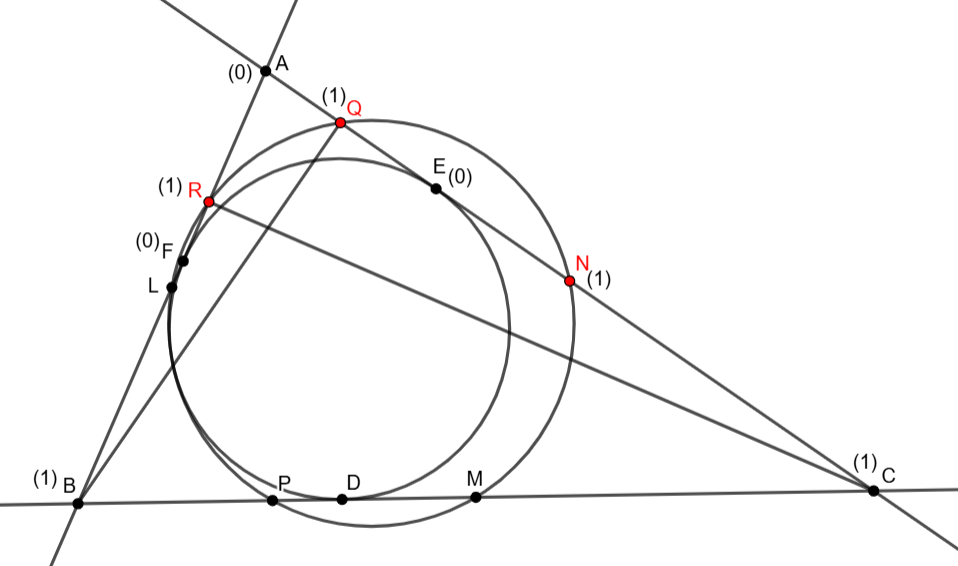
\includegraphics[width=0.8\textwidth]{kepek/feuerbach.png}
    \end{figure}

    Let the tangency points of the incircle be $D,E,F$ and the midpoints of the sides be $M,N,L$, see the figure.

    We will use incircle animation. Let's fix $A$, $E$, $F$ and the incircle, and start animating point $D$ with degree 2 on the incircle.

    As we saw it in the last example problem where we used the same animation, $\deg B=\deg C=1$.

    The feet of perpendicular to the fixed line $AB$ from $C$ is $R$, so $R$ has degree 1.

    Symmetrically $Q$ has degree one too.

    The midpoint $N$ has degree $0+1-0=1$. (There is a formula for midpoint not included in this paper)

    It is well known that the points $P,Q,R,M,N,L$ are all on the Feuerbach circle. In this case we define the F-circle as $(QRN)$.

    We can apply one of the previous theorem to calculate the degree of $(QRN)$:
    $$\deg (QRN)=2(\deg Q+\deg R+\deg N)-\#(\text{any two points are the same})-\#(\text{any point is one of the circle points})-$$
    $$-\#(\text{any 2 points are on the ideal line})-\#(\text{all 3 points are collinear on a line with slope $i$ or $-i$})=$$
    $$=2(1+1+1)-3-0-1-0=2$$

    Lets have a look at this in details. First calculate the coincidences. $Q$ and $N$ are degree 1 points on a fixed line, so they coincide exactly twice. When $C=A$, $N=R=A$ too, so $N$ and $R$ coincide once. And that is all.

    Secondly neither of the points $Q,R,N$ are any circle points, because they all lie on fixed lines with real slope.

    Thirdly when $C$ is an ideal point, then $N$ and $R$ are ideal points too, so $N$ and $R$ are in the ideal line at once.

    And lastly $Q,R$ and $N$ won't be collinear on a line with slope $i$ or $-i$.

    So the F-circle has degree 2, and the incircle is fixed.

    The statement "the F-circle is tangent to the incircle" has degree $2\deg (\text{F-circle})+2\deg (\text{incircle})=2\cdot 2+2\cdot 0=4$.

    So we need 5 cases where the statement is true, and we are done.

    \begin{enumerate}
        \item $AB=AC$: Here $D=P=M$, and both circles are symmetric the the axis, so they are tangent in $D=P=M$.
        \item $AB=AC$: The second such case.
        \item $BA=BC$: The triangle is isosceles in another way.
        \item $CA=CB$: Yet another isosceles case.
        \item $B$ is an ideal point: Here the F-circle degenerates into the union of line $NR$ and the ideal line. We are left to prove a simple elementary problem.
        \begin{figure}[H]
        \centering
        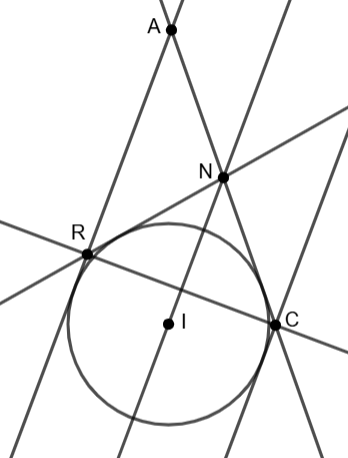
\includegraphics[width=0.25\textwidth]{kepek/feuerbach2.png}
        \end{figure}
        Now $AB$ and $CB$ are parallel lines. Let the parallel line halfway between them be $l$. $N$ is the middle point of $AC$, so it is on $l$. $I$ is the center of the incircle, which is tangent to both $AB$ and $CB$, so $I$ is also on $l$. $R$ is the foot of the altitude from $C$ to $AB$, now this is the mirror image of $C$ w.r.t. $l$. Therefore segments $NC$ and $NR$ are also mirror images w.r.t. $l$. Since $NC$ is tangent to the incircle, $NR$ must be tangent to it too. But line $NR$ is the degenerate F-circle, so we proved the statement.
    \end{enumerate}

\end{proof}
\subsection{Power of a point}

The power of a point with respect to a circle is a useful tool in geometry problems.

Given a circle $c$ with equation in the standard form $x^2+y^2+dx+ey+f=0$. Substituting $P=(x,y)$ we get the power of $P$ with respect to $c$.

\begin{theorem}
    Let $P$ be a polynomial moving point and let $c$ be a polynomial moving circle. Then the power $p^2$ of $P$ with respect to $c$ has degree at most

    $$\deg (p^2)\le\deg c+2\deg P-\#(\text{"$P$ is a circle point" or "$c$ splits into the ideal line and an other line, and $P$ is on $c$")}$$
\end{theorem}
\begin{proof}
    $P=(x:y:z)$ and $c=(A:B:C:D:E:F)$. The power is
    $$p^2=\frac{x^2}{z^2}+\frac{y^2}{z^2}+\frac{D}{A}\frac{x}{z}+\frac{E}{A}\frac{y}{z}+\frac{F}{A}$$
    With homogeneous coordinates in $\cc\pp^1$
    $$p^2=(Ax^2+Ay^2+Dxz+Eyz+Fz^2:Az^2)$$
    Both coordinates have degree $\deg c+2\deg P$, and we have to subtract when $p=(0,0)$.

    We have two options for this, one is $z=0$ and the other is $A=0$. When $A=0$, $Dxz+Eyz+Fz^2$ is the equation of the conic, which splits into $\{z=0\}$ and $\{Dx+Ey+Fz=0\}$, which are the ideal line an arbitrary line.
    When $z=0$, $Ax^2+Ay^2=0$, which can be by $A=0$ or by $P$ being one of the circle points.
\end{proof}


\begin{corollary}
    Let $c$ be a degree 2 moving circle. Then there exists a point $P$ whose power with respect to $c$ is constant.
\end{corollary}
\begin{proof}
    Take 3 positions of $c$ as time passes. There exists a point $P$ of which all 3 powers are the same. The power of $P$ with respect to $c$ has degree at most $0+2=2$, but now we found 3 times when it is constant, so it must be constant everywhere.
\end{proof}

\begin{theorem}
    Let $c_1$ and $c_2$ be two polynomial moving circles. Then their radical axis $r$ is polynomial and has degree at most
    $$\deg r\le \deg c_1+\deg c_2-\#(\text{"$c_1$ and $c_2$ splits into ideal line and some other line at the same time" or "$c_1=c_2$"})$$
\end{theorem}
\begin{proof}
    We attain the equation of the radical axis by subtracting the standard equations of $c_1$ and $c_3$:

    $$\left(\frac{x^2}{z^2}+\frac{y^2}{z^2}+\frac{D_1}{A_1}\frac{x}{z}+\frac{E_1}{A_1}\frac{y}{z}+\frac{F_1}{A_1}\right)-\left(\frac{x^2}{z^2}+\frac{y^2}{z^2}+\frac{D_2}{A_2}\frac{x}{z}+\frac{E_2}{A_2}\frac{y}{z}+\frac{F_2}{A_2}\right)=0$$
    Simplifying and multiplying by $A_1A_2z$:
    $$(D_1A_2-D_2A_1)x+(E_1A_2-E_2A_1)y+(F_1A_2-F_2A_1)z=0$$

    Therefore
    $$r=(D_1A_2-D_2A_1:E_1A_2-E_2A_1:F_1A_2-F_2A_1)$$

    So the radical axis has coordinates of degree $\deg c_1+\deg c_2$. We have to subtract when $r=(0,0,0)$. If $A_1=0$, then $D_1A_2=E_1A_2=F_1A_2=0$, and since $A_1$, $D_1$, $E_1$ and $F_1$ can't be all zero, $A_2=0$. If $A_2=0$, then $A_1=0$ symmetrically. If neither of them is zero, then $\frac{D_1}{A_1}=\frac{D_2}{A_2}$, $\frac{E_1}{A_1}=\frac{E_2}{A_2}$ and $\frac{F_1}{A_1}=\frac{F_2}{A_2}$, so the two circles are the same.
\end{proof}


Three circles are coaxial if they have two common intersection points, or if they are tangent in one common point.

\begin{theorem}
    Let $c_1$, $c_2$ and $c_3$ be three polynomial moving circles. Then their radical center $R$ is polynomial, and its degree is at most
    $$\deg R\le\deg c_1+\deg c_2+\deg c_3 -\#(\text{"the 3 circles are coaxial" or}$$
    $$\text{"$c_1$, $c_2$ and $c_3$ all split to the ideal line and some other line"})$$
\end{theorem}
\begin{proof}
    For each circle $c_i$ with equation
$$
x^2 + y^2 + \frac{D_i}{A_i} x + \frac{E_i}{A_i} y + \frac{F_i}{A_i} = 0,
$$
the quantity \(D_i x + E_i y + F_i\) has the same value for every \(i\) at the radical center. So there exists a scalar \(\lambda\) such that
$$
\frac{D_i}{A_i} x + \frac{E_i}{A_i} y + \frac{F_i}{A_i} = \lambda \qquad (i=1,2,3).
$$
or
$$D_i x + E_i y + F_i = \lambda A_i$$
That gives a \(3\times3\) linear system for the unknowns \(x, y, \lambda\):
$$
\begin{bmatrix}
D_1 & E_1 & -A_1\\[4pt]
D_2 & E_2 & -A_2\\[4pt]
D_3 & E_3 & -A_3
\end{bmatrix}
\begin{bmatrix}
x\\[4pt] y\\[4pt] \lambda
\end{bmatrix}
=
\begin{bmatrix}
-F_1\\[4pt] -F_2\\[4pt] -F_3
\end{bmatrix}.
$$
\noindent
Using Cramer’s rule you get
$$
x = \frac{\det A_x}{\det A}, \qquad
y = \frac{\det A_y}{\det A},
$$
where
$$
A_x =
\begin{pmatrix}
-F_1 & E_1 & -A_1\\[4pt]
-F_2 & E_2 & -A_2\\[4pt]
-F_3 & E_3 & -A_3
\end{pmatrix}, \qquad
A_y =
\begin{pmatrix}
D_1 & -F_1 & -A_1\\[4pt]
D_2 & -F_2 & -A_2\\[4pt]
D_3 & -F_3 & -A_3
\end{pmatrix}, \qquad
A =
\begin{pmatrix}
D_1 & E_1 & -A_1\\[4pt]
D_2 & E_2 & -A_2\\[4pt]
D_3 & E_3 & -A_3
\end{pmatrix}
$$

So in homogeneous coordinates $R=(\det A_x:\det A_y:\det A)$

All three coordinates are degree $\deg c_1+\deg c_2+\deg c_3$ polynomials. We have to subtract the number of times when $R=(0,0,0)$.

These determinants are $3\times 3$ subdeterminants of the matrix (possibly with different sign)

$$M =
\begin{pmatrix}
D_1 & E_1 & F_1 & A_1\\[4pt]
D_2 & E_2 & F_2 & A_2\\[4pt]
D_3 & E_3 & F_3 & A_3
\end{pmatrix}$$

%If 2 of the maximal subdeterminants are zero in a $n\times (n+1)$ matrix, then all of them are zero.

If $a=(A_1,A_2,A_3)=(0,0,0)$, then all three determinants are zero. This is equivalent to the condition "$c_1$, $c_2$ and $c_3$ all split to the ideal line and some other line"

If $a\ne 0$ then for $d=(D_1,D_2,D_3)$, $e=(E_1,E_2,E_3)$, $f=(F_1,F_2,F_3)$ we know that $\langle f,e,a\rangle$, $\langle d,f,a\rangle$ and $\langle d,e,a\rangle$ are all at most 2 dimensional subspaces of $\cc^3$. This is only possible if $a,d,e,f$ are all in one at most two dimensional subspace, ensuring that the 4th subdeterminant of $M$ is also 0.

So if $a\ne 0$ the condition $\det A_x=\det A_y=\det A=0$ is equivalent to $\mathrm{rk} M\le 2$.

This is equivalent to the rows of $M$ being linearly dependent, or that the vectors $c_i=(A_i,0,A_i,D_i,E_i,F_i)$ $i=1,2,3$ are linearly dependent. The orthogonal complement of $\langle c_1,c_2,c_3\rangle$ is then at least 3 dimensional. The $(x:y:z)\in \pp^2$ points for which $(x^2:xy:y^2:xz:yz:z^2)\in \pp^5$ is in this orthogonal complement are on all three circles. But $c_1$ and $c_2$ span the same subspace as $c_1$, $c_2$ and $c_3$ (suppose $c_1\ne c_2$), so as circles, the intersection of $c_1$ and $c_2$ is the same set as the intersection of $c_1$, $c_2$ and $c_3$. Which means that the 3 circles are coaxial. Or if $c_1=c_2$, the 3 circles are coaxial anyway.




\end{proof}


\subsection{Inversion}

\begin{theorem}
    Let $P$ be a polynomial moving point, and $c$ be a polynomial moving circle with center $O$. The inverse image of $P$ w.r.t. $c$ is $Q$. Then $Q$ is polynomial, and its degree is at most
    $$\deg Q\le2\deg P+2\deg c-\#(O=P)-\#(\text{"$P$ is one of the circle points" or}$$
    $$\text{"$c$ splits into two lines with slopes $i$ and $-i$, and $P$ is on $c$" or}$$
    $$\text{"$c$ splits into the ideal line and a line $l$, and $P$ is an ideal point" or}$$
    $$\text{"$c$ splits into the ideal line and a line $l$ with slope $i$ or $-i$ and $P$ is on $l$" or}$$
    $$\text{"$c$ is the ideal line counted twice"})$$
\end{theorem}

\begin{remark}
    If $c$ is fixed, the formula gets much more simple:

    $$\deg Q\le2\deg P-\#(\text{"$O=P$" or "$P$ is one of the circle points"})$$
\end{remark}

\begin{proof}
    $$P=(x:y:z)$$
    $$c=(A:0:A:D:E:F)$$
    Then the center $O$, and square of radius $r^2$ of $c$ is
    $$O=(D:E:-2A)$$
    $$r^2=\frac{D^2+E^2-4AF}{4A^2}$$
    We can give the position of $Q$ with euclidean vectors
    $$\vec{Q}=\vec{O}+\frac{r^2}{|OP|^2}\overrightarrow{OP}$$
    Substituting in, we get
    $$\vec{Q}=\left(\frac{D}{-2A},\frac{E}{-2A}\right)+\frac{\frac{D^2+E^2-4AF}{4A^2}}{\left(\frac{x}{z}-\frac{D}{-2A}\right)^2+\left(\frac{y}{z}-\frac{E}{-2A}\right)^2}\left(\frac{x}{z}-\frac{D}{-2A},\frac{y}{z}-\frac{E}{-2A}\right)$$
    Simplifying and homogenising:
    $$Q=(-2D(Ax^2+Ay^2+Dxz+Eyz+Fz^2)+(E^2+D^2-4AF)xz:$$
    $$-2E(Ax^2+Ay^2+Dxz+Eyz+Fz^2)+(E^2+D^2-4AF)yz:$$
    $$(2Ax+Dz)^2+(2Ay+Ez)^2)$$
    This may seem ugly, but it is manageable. All coordinates have degree $2\deg P+2\deg c$. We have to subtract from this the number of times when $Q=(0,0,0)$. There are several cases.

    If $A\ne 0$ and $z\ne0$ then we can factor out every coordinate by $4A^2z^2$. With $P=(p_1,p_2)=\left(\frac{x}{z},\frac{x}{z}\right)$, $O=(o_1,o_2)=\left(-\frac{D}{2A},-\frac{E}{2A}\right)$ and (power of $P$ w.r.t. $c) = p^2=p_1^2+p_2^2+\frac{D}{A}p_1+\frac{E}{A}p_2+\frac{F}{A}$ we get
    $$Q=(p^2o_1+r^2p_1:p^2o_2+r^2p_2:(p_1-o_1)^2+(p_2-o_2)^2)$$
    There is an identity $p^2=|OP|^2-r^2=(p_1-o_1)^2+(p_2-o_2)^2-r^2$. When $Q=(0,0,0)$, then $(p_1-o_1)^2+(p_2-o_2)^2=0$, and so $p^2=-r^2$. Therefore the first two coordinates of $Q$ are $r^2(p_1-o_1)$ and $r^2(p_2-o_2)$, which can be both zero if and only if $r=0$ or $P=O$. Conversely if $P=O$ then $Q=(0,0,0)$. Furthermore if $(p_1-o_1)^2+(p_2-o_2)^2=0$ or equivalently $P$ is on the circle with radius 0 and center $O$ (the union of lines with slope $i$ and $-i$ through $O$), then $r=0$ is sufficient for $Q=(0,0,0)$.

    If $A\ne 0$ and $z=0$ then the third coordinate of $Q$ is $4A^2(x^2+y^2)$, which is zero if and only if $x^2+y^2=0$. But then the first two coordinates are automatically zero too. So $Q=(0,0,0) \iff z=0$ and $x^2+y^2=0 \iff P$ is one of the circle points.

    If $A=0$ and $z\ne0$ then the third coordinate of $Q$ is zero if and only if $D^2+E^2=0$. But then the first two coordinates of $Q$ simplify to $D(Dx+Ey+Fz)$ and $E(Dx+Ey+Fz)$. These are zero iff $D=E=0$ or $Dx+Ey+Fz=0$. So here $Q=(0,0,0)$ iff $c$ splits into a the ideal line and a line $l$ with slope $i$ or $-i$, and $P$ is on $l$, or $c$ is the ideal line counted twice.

    If $A=0$ and $z=0$ then $Q=(0,0,0)$ trivially. This is equivalent to $c$ splitting into the ideal line and a line, and $P$ is on the ideal line.
\end{proof}

\begin{theorem}
    Let $c$ be a polynomial moving circle and $\omega$ a fixed circle. The inverse image of $c$ w.r.t. $\omega$ is $c'$. Then $c'$ is a polynomial moving circle, and its degree is the same as the degree of $c$.
\end{theorem}
\begin{proof}
    We will first give a proof when $\omega$ is the unit circle. Let $c=(A:0:A:D:E:F)$. The inverse image of a point $(x:y:z)$ w.r.t. the unit circle is $(xz:yz:x^2+y^2)$. The points on $c'$ are exactly the points whose inverse image is on $c$. Therefore we obtain the equation of $c'$ by substituting $(xz:yz:x^2+y^2)$ into the equation of $c$, that is
    $$A(xz)^2+A(yz)^2+Dxz(x^2+y^2)+Eyz(x^2+y^2)+F(x^2+y^2)^2=0$$
    Simplifying by $x^2+y^2$:
    $$Az^2+Dxz+Eyz+F(x^2+y^2)=0$$
    So $c'=(F:0:F:D:E:A)$, and it has the same degree as $c'$.

    When $\omega$ is a general circle, we can take a homothety that takes $\omega$ to the unit circle, then invert w.r.t. the unit circle, then take the inverse of the homothety, and in the end we get the desired inverse image w.r.t. $\omega$. Using that homotheties preserve degree, $\deg c=\deg c'$.
\end{proof}

\section{Square root moving points}


It naturally comes up in geometry problems to calculate the degree of the intersection of a polynomial moving line and a fixed conic. However unlike all previous cases, these intersection points are not necessarily polynomial. They are so-called `square root points'. Their homogeneous coordinates are in the following set:

Let $\cc\Bigl[t,s,\sqrt{H}\Bigr]_h=\Bigl\{a+b\sqrt{H}\mid a,b\in \cc[t,s]_h,\quad \deg a=\deg b+r\Bigr\}$, where $H\in \cc[t,s]_h$, such that $H$ is not a square of any polynomial, and $\deg H=2r$ for an $r\in \nn$.

\begin{lemma}
    $\cc\Bigl[t,s,\sqrt{H}\Bigr]_h$ contains the homogeneous elements of a graded ring with index set $\{r,r+1,\ldots\}$, such that an element $a+b\sqrt{H}$ has degree $\deg a$.
\end{lemma}
\begin{proof}
    $$\left(a+b\sqrt{H}\right)+\left(c+d\sqrt{H}\right)=(a+c)+(b+d)\sqrt{H}$$
    Therefore adding two element with the same degree creates a third element with that degree.
    $$\left(a+b\sqrt{H}\right)\left(c+d\sqrt{H}\right)=(ac+bdH)+(bc+ad)\sqrt{H}$$
    $\deg (ac)=\deg (bdH)=\deg (bc+ac)+r$, therefore multiplying two elements of degree $p$ and $q$ creates an element with degree $p+q$.
\end{proof}

Let $\cc\Bigl[t,s,\sqrt{H}\Bigr]_h^d$ denote the set of degree $d$ elements in $\cc\Bigl[t,s,\sqrt{H}\Bigr]_h$.



\begin{definition}
    $a+b\sqrt{H}$ and $a-b\sqrt{H}$ are conjugate pairs, the conjugate of $p \in \cc\Bigl[t,s,\sqrt{H}\Bigr]_h$ is denoted $\overline{p}$.
\end{definition}
\begin{lemma}
    This conjugation is an automorphism of $\cc\Bigl[t,s,\sqrt{H}\Bigr]_h$.
\end{lemma}
\begin{proof}
    It is an automorphism of $\cc\Bigl[t,s,\sqrt{H}\Bigr]$ (allowing non-homogeneous elements), because $\sqrt{H}$ and $-\sqrt{H}$ have the same minimal polynomial: $x^2-H=0$, so there exists an automorphism fixing $\cc[t]$, and taking $\sqrt{H}$ to $-\sqrt{H}$. That must be the above defined conjugation.
    Now $\cc\Bigl[t,s,\sqrt{H}\Bigr]_h$ is closed to conjugation, so the conjugation is also an automorphism of this subset.
\end{proof}

\begin{remark}
    $\sqrt{H}$ isn't well defined, only $\pm \sqrt{H}$ as a 2-valued function. The elements of $\cc\Bigl[t,s,\sqrt{H}\Bigr]_h$ are also not well defined, but from now on we only use expressions that are symmetric with respect to conjugation at the actual method, and these are well defined, and we only use the expressions that are not symmetric formally.
\end{remark}


Conjugate pair square root valued functions also have multiplicity analogous to the polynomial version.
$$\ord_t\Bigl(\left(f,\overline{f}\right)\Bigr)=\frac{\ord_t(f\cdot \overline{f})}{2}$$
$f\cdot\overline{f}$ is symmetric to conjugation, so it is necessarily a polynomial.
Square root multiplicity is always a half-integer.


\begin{definition}

    An ordered pair of moving points $(P_1, P_2)$ is a \textit{square root point pair} if there exist $p_0,...,p_n \in \cc\Bigl[t,s,\sqrt{H}\Bigr]_h^d$ such that $$\big(P_1(t:s), P_2(t:s)\big)=\big((p_0(t,s):\ldots:p_n(t,s)), (\overline{p_0}(t,s):\ldots:\overline{p_n}(t,s))\big)$$

    with homogeneous coordinates.

    The \textit{degree} of the square root point pair is
    $$d-\frac{\#\bigl(|(p_0,\ldots,p_n)|=0\text{ or } |(\overline{p_0},\ldots,\overline{p_n})|=0\bigr)}{2}$$
    where $\#\bigl(|(p_0,\ldots,p_n)|=0\text{ or } |(\overline{p_0},\ldots,\overline{p_n})|=0\bigr)$ is taken with multiplicity.

    When $(p_0,\ldots,p_n)=0$, $P_1$ is defined as $\frac{(p_0,\ldots,p_n)}{|(p_0,\ldots,p_n)|}$, $P_2$ similarly.

    We call $(p_0:\ldots:p_n)$ a polynomial format of $(P_1, P_2)$.
\end{definition}

\begin{lemma}
    Degree is well defined, and always a positive half-integer.
\end{lemma}
\begin{proof}
    The square root point-line theorem states that a square root point pair passes through a fixed line exactly 2 times the degree of the point pair, so the degree must only depend on the moving point pair as a function and not on its polynomial format. It follows that degree is a positive half-integer too.
\end{proof}
We can define moving line pairs the same way as moving point pairs.
\begin{remark}
    A polynomial moving point/line of degree $n$ paired with itself form a square root point/line pair of degree $n$.
\end{remark}

\subsection{Intersection of a moving line and a fixed conic}

\begin{theorem}
    The two (not necessarily different) moving intersection points of a polynomial moving line of degree $n$ and a fixed conic either form a square root point pair of degree $n$ or they are both polynomial.

    % of the form $$P,Q=\left(a\pm b\sqrt{H}:c\pm d\sqrt{H}:e\pm f\sqrt{H}\right)$$
    % where both sides are 2-valued functions (hence the $\pm)$, and $a,b,c,d,e,f,H \in \cc[t]$, or both $P$ and $Q$ are polynomial points.
\end{theorem}
\begin{proof}
    We want to prove that every coordinate is in $\cc\Bigl[t,s,\sqrt{H}\Bigr]_h^d$ for some $H$ and $d$, and also that $P$ and $Q$ are conjugate pairs, and also that it is degree $n$. A projective transformation keeps this square root form, the conjugate relation and the degree, because it only uses ring operations. So we can suppose that the conic is the origin-centered, radius 1 circle. Let $l:(A:B:C)$ be a degree $n$ polynomial moving line. Then $Ax+By+C=0$ is the equation of the line, and $x^2+y^2=1$ is the equation of the circle.

    From the line equation $y=\frac{-C-Ax}{B}$

    Substituting this into the circle equation gives us $$x^2+\left(\frac{-C-Ax}{B}\right)^2=1 \iff (A^2+B^2)x^2+(2AC)x+(C^2-B^2)=0$$

    $$x_{1,2}=\frac{-AC\pm \sqrt{A^2C^2-(C^2-B^2)(A^2+B^2)}}{A^2+B^2}=\frac{-AC\pm B\sqrt{A^2+B^2-C^2}}{A^2+B^2}$$

    Doing the same with $y$:

    $$y_{1,2}=\frac{-BC\pm A\sqrt{A^2+B^2-C^2}}{A^2+B^2}$$

    In homogeneous coordinates:

    $$P=(-AC + B\sqrt{A^2+B^2-C^2}:-BC - A\sqrt{A^2+B^2-C^2}:A^2+B^2)$$
    $$Q=(-AC - B\sqrt{A^2+B^2-C^2}:-BC + A\sqrt{A^2+B^2-C^2}:A^2+B^2)$$

    Taking $H=A^2+B^2-C^2$, if $H$ the square of some polynomial, then both $P$ and $Q$ are polynomial points, and if $H$ is not the square of some polynomial, then the coordinates are indeed in $\cc\Bigl[t,s,\sqrt{H}\Bigr]_h^{2n}$ with a conjugate relation.

    The degree of a point pair $(p_0,p_1,p_2), (\overline{p_0}, \overline{p_1}, \overline{p_2})$ is the half the degree of the polynomial point $(p_0\overline{p_0}, p_1\overline{p_1}, p_2\overline{p_2})$.
    In this case that is
    $$\bigl((AC)^2-B^2(A^2+B^2-C^2):(BC)^2-A^2(A^2+B^2-C^2):(A^2+B^2)^2\bigr)=$$
    $$=\bigl((A^2+B^2)(C^2-A^2):(A^2+B^2)(C^2-B^2):(A^2+B^2)^2\bigr)=$$
    $$=\bigl(C^2-A^2:C^2-B^2:A^2+B^2\bigr)$$
    This is never all zero, otherwise $(A,B,C)$ would be all zero, therefore this is a degree $2n$ point, so $(P,Q)$ is of degree $n$.
\end{proof}

\begin{theorem}[Polynomial intersection theorem]\label{polyinttheo}
    Let $l$ be a moving line, and $c$ be a fixed conic. If at every time, when $l$ becomes tangent to $c$, this happens with an even l-c multiplicity, then the intersections of $l$ and $c$ are two polynomial points.
\end{theorem}

\begin{proof}
\hfill \break
    Lemma 1: Let $f$ be a holomorphic function, which is not constant zero. Then the following are equivalent:
    \begin{enumerate}
        \item $f$ has even order of zero at $t_0$
        \item There exists a holomorphic $g$, such that $g^2=f$ at a neighborhood of $t_0$
    \end{enumerate}

    $1. \impliedby 2.$
    If $g$ has order of zero $a$, $f=g^2$ has order of zero $2a$.

    $1. \implies 2.$
    $f=t^{2a}\cdot h$, where $h$ is a holomorphic function, that is not zero at $t_0$.
    Since $t_0$ is not a limes point of zeros of $f$, there exists a neighborhood, where h has no zeros. Here exists a holomorphic $j$, such that $j^2=h$. Then $g=t^a\cdot j$ is a holomorphic function, such that $g^2=f$ at this neighborhood.



    Lemma 2: If $l$ is tangent to $c$ at some $t_0$, and the tangency has even l-c multiplicity, then the two intersection points are holomorphic at $t_0$.

    Let the tangency point of $l$ on $c$ at $t_0$ be $T$.

    With a projective transformation send $T$ to the Origin, and $c$ to the $x^2=y$ parabola.

    Projective transformations don't change multiplicities and holomorphicness.

    Let $A$ be the intersection of the y-axis and $l$.
    At a time near $t_0$, $A$ is of distance $a$ from the x-axis, and $l$ has slope $s$.

    \begin{figure}[H]
    \centering
    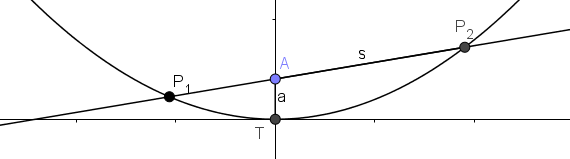
\includegraphics[width=0.7\textwidth]{kepek/conic-line.PNG}
    \end{figure}

    Since $l$ is the x-axis at $t_0$, $s$ convergates to 0, so $plmul(l,T)=plmul(A,x-axis)$ (the distances has ratio covergating to 1). Therefore $a$ also has even order of zero.

    We can calculate the $x$ coordinates of the intersections:

    $$y=x^2=a+sx$$
    $$x_{1,2}=\frac{s \pm \sqrt{s^2+4a}}{2}$$

    $s^2+4a$ is a holomorphic function, and since both $s^2$ and $4a$ has even order of zero, $s^2+4a$ has so. From Lemma 1, there exist two holomorphic functions $\pm g$, such that $(\pm g)^2=s^2+4a$. Therefore the $x$-coordinates are holomorphic functions at $t_0$. $y_{1,2}=x_{1,2}^2$, meaning that the $y$-coordinates are also holomorphic at $t_0$, so the intersection points are holomorphic at $t_0$.
    We proved Lemma 2.


    The homogeneous coordinates of the intersections of a polynomial line $l$, and a fixed conic $c$ are in $\cc\Bigl[t,s,\sqrt{H}\Bigr]_h$.
    Take a case when $H(t,s)=0$, $P_1=P_2$ and $l$ is tangent to $c$.

    Suppose $(t:s)$ is on the first chart of $\cc\pp^1$ (similarly works if it is on the second chart). In a neighbourhood of $(t:s)$ the intersection points can be written in the form
    $$P_{1,2} = \left(a \pm b\sqrt{h} , c \pm d\sqrt{h}\right)$$
    where $a,b,c,d\in \cc(t), h\in \cc[t]$, $h(t)=H(t,1)$, and the coordinates are meant according to the chart of $T$.

    Now $l$ is tangent to $c$, so from the condition and Lemma 2 $P_1$ and $P_2$ are holomorphic at $t_0=\frac{t}{s}$. This means that one of their coordinates, for example $a + b\sqrt{h}$ is holomorphic at $t_0$, and with some operations we get that $\pm\sqrt{b^2h}$ are holomorphic at $t_0$. From Lemma 1, $b^2h$ has an even order of zero at $t_0$, and thus $h$ has so. This means that $H$ has even order of zero at $(t:s)$.
    We conclude that every zero of $H$ (except the origin) is of even order, and so $H=G^2$, where $G\in\cc[t,s]_h$.

    So the intersections are polynomial points.
\end{proof}

\begin{theorem}
    Let $P$ be a moving point, and $c$ be a fixed conic. If at every time, when $P$ lies on $c$, this happens with an even multiplicity, then the tangents from $P$ to $c$ are two polynomial lines.
\end{theorem}

\begin{proof}
    The tangency points of the tangent lines from $P$ are $X$ and $Y$. $XY$ is the polar of $P$, and by Lemma ~\ref{polepolar mul} $\quad plmul(XY,T)=plmul(P,t)$, where $T$ is the arrival point of $P$ on $c$, and $t$ is the tangent line to $c$ at $T$. We know that both multiplicities are even. Then by the previous theorem, $X$ and $Y$ are polynomial, and the tangent lines are so.
\end{proof}


\subsection{Constructing further square root points}

In the polynomial case, we calculated the degree of a an object coming from a polynomial construction step. We'll see that if we apply the same construction step to square root object pairs, we get a new square root object pair. Furthermore, we can calculate its degree with the same formula as in the polynomial case. The next lemma makes this precise.

\begin{lemma}
    Suppose each $(X_{i1}, X_{i2})$ ($0\le i\le k)$ is a square root moving object pair of degree $d_i$.
    Let $Y$ be a polynomial construction step with homogeneity factors $\alpha_i$ and homogeneous polynomials $f_0,\ldots f_n$. Then $\tilde{Y}(X_1,\ldots,X_k)$ is also a polynomial moving object with degree
    $$\deg \tilde{Y}=\sum_{i=1}^k \alpha_id_i-\#(Y=(0,\ldots,0))$$
    where $\#(Y=(0,\ldots,0))$ counts the number of times when $Y=(f_0,\ldots ,f_n)=(0,\ldots,0)$. This is counted with multiplicity, which means the minimum order of zero among $f_0,\ldots, f_n$ as polynomials of time.
\end{lemma}
\begin{proof}
    Every $X_i$ object is polynomially moving, and has degree $d_i$. Then each variable $x_{i0},\ldots ,x_{im_i}$ is a degree $d_i$ polynomial of time.

    Then for every $j$, $f_j(x_{10},\ldots ,x_{km_k})$ is also a polynomial of time that has degree $\sum_{i=1}^k \alpha_id_i$.

    But we need to be careful, because there may be times $(t_0:s_0)$ where $Y=(0,\ldots,0)$, which is not allowed in the definition of a polynomial moving object. Fortunately, in this case we can factor out $(s_0t-t_0s)$ from all $f_0,\ldots, f_n$, and then divide homogenously by $(s_0t-t_0s)$. This way all the polynomials will have one less degree, and the order zero at $(t_0:s_0)$ of every $f_j$ will reduce by one too.

    We repeat this process until there are no cases where $Y=(0,\ldots,0)$. Then all polynomials will have degree $\sum_{i=1}^k \alpha_id_i-\#(Y=(0:\ldots:0))$, and they won't have common root. So the result will be a polynomial moving object with this degree.
\end{proof}












\begin{lemma}
    Every geometric construction that uses only field operations constructs only square root point/line pairs from square root point/line pairs.
\end{lemma}
\begin{proof}
    Such transformations can be expressed with homogeneous coordinates using multiplication, and addition. Therefore all coordinates stay in the set $\cc\Bigl[t,s,\sqrt{H}\Bigr]$ (allowing non-homogeneous elements). But the new point/line is well-defined in terms of time, so choosing $(\lambda t, \lambda s)$ instead of $(t,s)$ must change all three coordinates by the same multiplier, so they are homogeneous by the same degree, thus they are in $\cc\Bigl[t,s,\sqrt{H}\Bigr]_h^d$ for some $d$.
\end{proof}

\begin{corollary}
    projective transformation, pole-polar, line trough two points, intersection of two lines, affine combination of some points, inversion about any conic all construct only square root point/lines pairs from square root point/lines pairs. (Basically any construction step that comes up in olympiad geometry)
\end{corollary}
\begin{definition}
    When a geometric construction creates a square root point/line pair from polynomial points/lines, it is called a \textit{bipartition}. The product pair is called \textit{biparted pair}.
\end{definition}
\begin{example}
    The following are square root object pairs (or two polynomial objects):
    \begin{enumerate}
        \item The intersections of a polynomial moving line and a fixed conic
        \item The two tangents from a polynomial moving point to a polynomial moving conic
        \item The two angle bisectors of two polynomial moving lines
        \item The two intersections of a polynomial moving line and a polynomial moving circle
        \item The complex distance of two polynomial moving points: $$cdist(P,Q)=\pm\sqrt{(p_1-q_1)^2+(p_2-q_2)^2}$$
    \end{enumerate}
\end{example}


\begin{definition}
    Two square root points/lines are \textit{geometrically conjugate} if they can be constructed from a biparted pair using only field operations in a logical symmetric way, that is if we swap the role of the two points/lines of the biparted pair, the constructed points/lines also swap.
\end{definition}
\begin{example}
    Let $A$ be a polynomial moving point somewhere, and $P$ an $Q$ are the intersections of a moving line a fixed conic. Then lines $AP$ and $AQ$ are geometrically conjugate, because if we swap the roles of $P$ and $Q$, $AP$ and $AQ$ also swap.
\end{example}

\begin{lemma}
    Two geometrically conjugate points/lines also form a square root point/line pair.
\end{lemma}

\begin{proof}
    The biparted points/lines are both geometrically and algebraically conjugate. From them we construct geometrically conjugate points/lines only using ring operations on their homogeneous coordinates. Therefore the coordinates of these points/lines will be algebraically conjugate, since algebraic conjugation is an automorphism.
\end{proof}

\begin{lemma}
    A square root point/line that can be constructed from a biparted pair using only field operations, and that is logically symmetric to the biparted pair is a polynomial point/line.
\end{lemma}
\begin{example}
    The midpoint of the intersections of a moving line a fixed conic is polynomial.
\end{example}
\begin{proof}
    The point/line is its own geometric conjugate, so the coordinates of the point/line are also their own conjugates, so the coefficient of $\sqrt{H}$ is zero in them, and only polynomials remain.
\end{proof}

\subsection{Square root multiplicities}
We have seen in the polynomial part that multiplicity can be defined algebraically and can be calculated from the polynomial formats of the moving objects, or multiplicity can be defined geometrically, and it can be calculated from the moving object itself (as a function of time).
We can also define all types of multiplicities mentioned in the polynomial part for square root point pairs.
For example, the p-l multiplicity of a point pair and a line pair $(P_1,P_2)$ and $(l_1,l_2)$ is
$$plmul_t((P_1,P_2),(l_1,l_2))=\frac{\ord(dist(P_1,l_1)\cdot dist(P_2,l_2))}{2}$$
or equivalently the algebraic definition:
$$plmul_t((P_1,P_2),(l_1,l_2))=\frac{\ord\Bigl(\bigl(p_1\cdot l_1\bigr)\cdot \bigl(p_2\cdot l_2\bigr)\Bigr)}{2}-\frac{\ord\bigl(p_1=0\bigr)+\ord\bigl(p_2=0\bigr) +\ord\bigl(l_1=0\bigr)+\ord\bigl(l_2=0\bigr)}{2}$$
where $p_1,p_2,l_1,l_2$ vectors are the polynomial formats of $P_1,P_2,L_1,L_2$ respectively.

The algebraic and the geometric definitions are equivalent, because $$\ord\Bigl(dist(P_1,l_1)\Bigr)=\ord\left(\frac{p_1\cdot l_1}{|p_1|\cdot |l_1|}\right)$$

Similarly we can define every multiplicity analogously.

Multiplicity is always a half-integer.

\subsection{Square root degree of statements}

In the polynomial case, a degree $n$ polynomial statement about polynomial objects (points/lines/quantities) is either true $n$ times with multiplicity, or it is always true. This means that
$$\sum_{t\in\cc\pp^1} \operatorname{mul}_t(\text{"statement"})$$
is either $n$ or the statement is always true.

The statement can be stated about square root pairs too. In this case, we have a statement $s_1$ about one object from each pair, and we have another statement $s_2$ about the other half of each pair. $s_2$ is called the conjugate statement of $s_1$. In this case $s_1$ and $s_2$ are called square root statement pairs.

For example if we have a square root point and line pair $(P_1,P_2)$ and $(l_1,l_2)$, the statements "$P_1$ is on $l_1$" and "$P_2$ is on $l_2$" form a square root statement pair.

Denote the geometric multiplicity of $S_1$ and $S_2$ by $\operatorname{mul}_t(S_1)$ and $\operatorname{mul}_t(S_2)$ respectively.

The multiplicity of a square root statement pair at a time $t$ can be defined as
$$\operatorname{mul}_t(S_1,S_2)=\frac{\operatorname{mul}_t(S_1)+\operatorname{mul}_t(S_2)}{2}$$

This is best to remember as the "average multiplicity", since it counts an average of the multiplicity of $S_1$ and $S_2$.

We define the degree of a square root statement pair as $$\deg (S_1,S_2)=\sum_{t\in\cc\pp^1} \operatorname{mul}_t(S_1,S_2)$$

In the polynomial case we had Lemma ~\ref{degst}, and similarly we have a square root version of this Lemma:

Recall, that a \textit{polynomial} statement $S$ about objects $X_1,\ldots, X_k$ can be defined as a polynomial construction step to $\cc^1$.
$$(x_{10},\ldots,x_{1m_1}),\ldots,(x_{k0},\ldots,x_{km_k})\mapsto f(x_{10},\ldots ,x_{km_k})$$
where for every $i$, $f$ is homogeneous in $x_{i0},\ldots,x_{im_i}$ with homogeneity factors $\alpha_i$, just as in the definition of a polynomial construction step.

\begin{lemma}
    Suppose each $(X_{i1}, X_{i2})$ ($0\le i\le k)$ is a square root moving object pair of degree $d_i$. Let $S$ be a polynomial statement with homogeneity factors $\alpha_i$, and homogeneous polynomial $f$. Let $S_1$ and $S_2$ be the statement $S$ about $\{X_{i1}\}$ and $\{X_{i2}\}$ respectively. Then $S_1$ and $S_2$ form a square root statement pair with degree
    $$\deg (S_1,S_2)=\sum_{i=1}^k \alpha_id_i$$
    or "$S_1$ or $S_2$" is always true.
\end{lemma}
\begin{proof}
    Every $(X_{i1}, X_{i2})$ is a square root object pair, and has degree $d_i$. Therefore they can be written as $$X_{i1}=(x_{i0}:\ldots:x_{im_i})$$
    $$X_{i2}=(\overline{x_{i0}}:\ldots:\overline{x_{im_i}})$$
    where $x_{i0}:\ldots:x_{im_i} \in \cc\Bigl[t,s,\sqrt{H}\Bigr]_h^{d'_i}$, and $d'_i=d_i+\frac{\#\bigl(|(x_{i0}:\ldots:x_{im_i})|=0\text{ or } |(\overline{x_{i0}}:\ldots:\overline{x_{im_i}})|=0\bigr)}{2}$.



    We know that $f$ is a homogeneous polynomial with homogeneity factors $\alpha_i$, therefore $f(x_{10},\ldots,x_{km_k})$ and $f(\overline{x_{10}},\ldots,\overline{x_{km_k}})$ form a square root conjugate pair of degree $\sum_{i=1}^k \alpha_id'_i$.

    Since

    Therefore $f$ is either the constant zero polynomial, in which case the statement is always true, or it has exactly $\sum_{i=1}^k \alpha_id_i$ roots with multiplicity.

    We are done, because $\#(\text{"$S$ is true"})$ counts the roots of $f$ with multiplicity.
\end{proof}


\begin{theorem}
    Let $(s_1, s_2)$ be a square root statement pair. Then
\end{theorem}






\begin{definition}
    The degree of a statement about point/line pairs $(A_1,B_1),\ldots, (A_k,B_k)$ with a certain multiplicity is
    $$\sum_{t\in\cc\pp^1} \operatorname{mul}_t((A_1,B_1),\ldots, (A_k,B_k))$$
\end{definition}

% An element $r\in \cc\Bigl[t,s,\sqrt{H}\Bigr]_h$ is associated with the statement such that $mul(\text{statement})=\frac{\ord(r\overline{r}=0)}{2}$. The degree of the statement is $\deg r$.

The degree of statements can be used in the following way:

\begin{theorem}
    A degree $n$ statement about point/line pairs $(A_1,B_1),\ldots, (A_k,B_k)$ is true for either $A_1,\ldots, A_k$ or $B_1,\ldots, B_k$ exactly $2n$ times with multiplicity.
\end{theorem}
\begin{proof} $$2n=2\cdot\sum_{t\in\cc\pp^1} mul_t((A_1,B_1),\ldots, (A_k,B_k))=\sum_{t\in\cc\pp^1} mul_t(A_1,\ldots, A_k)+\sum_{t\in\cc\pp^1} mul_t(B_1,\ldots, B_k)$$
\end{proof}

\begin{theorem}[Square root point-line theorem]
    Let $(P_1,P_2)$ be a square root point pair, and let $(l_1,l_2)$ be a square root line pair. Then the degree of the statement "$P_1$ is on $l_1$ or $P_2$ is on $l_2$" (with sqrt point-line multiplicity) is exactly $\deg (P_1,P_2)+ \deg (l_1,l_2)$.
\end{theorem}
\begin{proof}
    Let $p_1,p_2,l_1,l_2$ vectors be the polynomial formats of $P_1,P_2,L_1,L_2$ respectively.
    $$\sum_{t\in\cc\pp^1}plmul_t((P_1,P_2),(l_1,l_2))=$$
    $$=\sum_{t\in\cc\pp^1}\frac{\ord\Bigl(\bigl(p_1\cdot l_1\bigr)\cdot \bigl(p_2\cdot l_2\bigr)\Bigr)}{2}-\sum_{t\in\cc\pp^1}\frac{\ord\bigl(p_1=0\bigr)+\ord\bigl(p_2=0\bigr) +\ord\bigl(l_1=0\bigr)+\ord\bigl(l_2=0\bigr)}{2}=$$
    $$=\deg p_1+\deg l_1-\frac{\#\bigl(p_1=0\text{ or } p_2=0\bigr)}{2}-\frac{\#\bigl(l_1=0\text{ or } l_2=0\bigr)}{2}=\deg (P_1,P_2)+ \deg (l_1,l_2)$$
\end{proof}
And analogously every degree of statement type theory works the same way as in the polynomial case.

\subsection{Square root versions of further theorems}

In fact every geometric construction is calculated the same way as in the polynomial case.

For example
\begin{theorem}
    Let $\mathcal{A}$ be a projective transformation, $(P_1,P_2)$ a square root point pair, and $(l_1,l_2)$ a square root line pair. Then $\deg (P_1,P_2)=\deg (\mathcal{A}(P_1),\mathcal{A}(P_2))$ and $\deg (l_1,l_2)=\deg (\mathcal{A}(l_1),\mathcal{A}(l_2))$
\end{theorem}
\begin{proof}
    Let $A$ be the nonsingular matrix of $\mathcal{A}$. Let $p$ be the polynomial format of $(P_1,P_2)$. Then $Ap$ consists of the linear combinations of the elements of $p$, so they are of the same degree as the elements of $p$. And also $\ord(|p|)=\ord(|Ap|)$.
    So $$\deg(P_1,P_2)=\deg p-\ord(|p|)=\deg Ap-\ord(|Ap|)=\deg (\mathcal{A}(P_1),\mathcal{A}(P_2))$$
    Similarly with $(l_1,l_2)$.
\end{proof}

An other example:
\begin{theorem}[Sqrt L-pp theorem]
    Let $(P_1,P_2)$ and $(Q_1,Q_2)$ be two square root point pairs. Then the degree of square root line pair $(P_1Q_1, P_2Q_2)$ is

$$\deg (P_1Q_1, P_2Q_2)= \deg (P_1,P_2) + \deg (Q_1,Q_2) - \# ((P_1,P_2)=(Q_1,Q_2))$$

where $\# ((P_1,P_2)=(Q_1,Q_2))$ denotes half the number of times $t\in \cc\pp^1$ when $P_1=Q_1$ or $P_2=Q_2$ (with square root point-point multiplicity).\\
\end{theorem}
\begin{proof}
    For any three point pairs $(A_1,A_2)$, $(B_1,B_2)$ and $(C_1,C_2)$
    $$3pmul_{t_0}((A_1,A_2),(B_1,B_2),(C_1,C_2))=plmul_{t_0}((C_1,C_2),(A_1B_1,A_2B_2))+ppmul_{t_0}((A_1,A_2),(B_1,B_2))$$
    That's because for all types of multiplicities $$mul((A_1,A_2),(B_1,B_2),(C_1,C_2))=\frac{mul(A_1,B_1,C_1)+mul(A_2,B_2,C_2)}{2}$$
    and for the ordinary form of these multiplicities the above equation holds.

    The rest of the proof goes the same way as the original proof of the L-pp theorem ~\ref{l-pp}.
\end{proof}

\begin{example}
    The intersections of a fixed circle $c$ and a degree 1 polynomial moving line $l$ are $A$ and $B$. $F$ is a fixed point on $c$. The lines $FA$ and $FB$ form a square root line pair of degree $0+1-\frac{1}{2}=\frac{1}{2}$. $F=A$ or $B$ happens one time, when line $l$ passes through $F$. Here exactly one of $A$ and $B$ coincides with $F$, so on average $A$ and $B$ coincide with $F$ $\frac{1}{2}$ times.
    \begin{figure}[H]
    \centering
    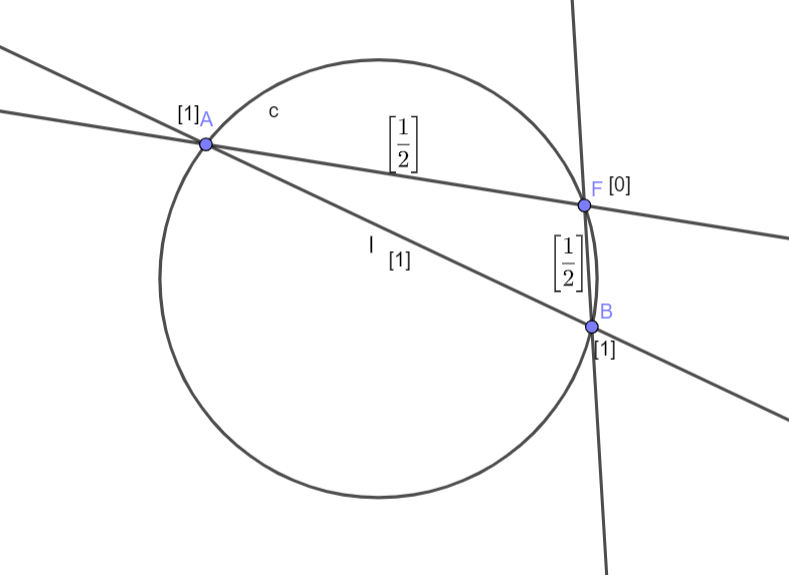
\includegraphics[width=0.7\textwidth]{kepek/sqrtllpex.png}
    \end{figure}
\end{example}

\begin{theorem}[Square root Locus theorem]
    A degree $\frac{n}{2}$ square root point $P$ and $\overline P$ are always moving on a shared degree $k$ algebraic curve, where $k\mid n$, furthermore for every smooth point $A$ of the curve, $P$ and $\overline P$ together pass through $A$ $\frac{n}{k}$ times (with p-p mul.). For every order $d$ singularity $B$, $P$ and $\overline P$ together pass through $B$ $\frac{n}{k}\cdot d$ times (with p-p mul.)
\end{theorem}
\begin{proof}
    The proof of the polynomial Locus theorem ~\ref{locus} can be rephrased to the square root language.

    Analogously $P=(p,q,r)$ moves on an algebraic curve. That is
    $$\sum a_ip^aq^br^c=0$$
    Taking the conjugate of both sides
    $$\sum a_i\overline{p}^a\,\overline{q}^b\,\overline{r}^c=0$$
    So $\overline{P}$ also moves on that same algebraic curve.

    The only nontrivial change in the proof is that all points where $H(t)=0$ are also defined as problematic, because then $P$ is not holomorphic. Otherwise it is, and the proof goes on all right.
\end{proof}

Square root Mászó-theorem can also be proven analogously.

\begin{lemma}
    If a square root point pair moves on a conic, it has integer degree.
\end{lemma}
\begin{theorem}[Sqrt Mászó-theorem]
Two square root point pairs $(A_1,A_2)$ and $(B_1,B_2)$ move on the same conic. Then
$$\deg (A_1B_1,A_2B_2) = \frac{\deg (A_1,A_2)+\deg (B_1,B_2)}{2}$$

\end{theorem}

\begin{theorem} [Inverse of Sqrt Mászó-theorem]

    Let $\mathcal{C}$ be a fixed conic, $(A_1,A_2)$ a square root point pair on it, and $(l_1,l_2)$ a square root line pair such that $l_1$ and $l_2$ always goes through $A_1$ and $A_2$ respectively. The second intersection of $\mathcal{C}$ and $l_1$ and $l_2$ is $B_1$ and $B_2$ respectively. Then $(B_1,B_2)$ form a square root point pair, and its degree satisfies

    $$\deg (l_1,l_2) = \frac{\deg (A_1,A_2)+\deg (B_1,B_2)}{2}$$

\end{theorem}


\section{Example problem for square root animation}

\begin{exercise}[Poncelet-porism]
    Let $C$ and $D$ be two conics, such that there exists a polygon with $n$ sides inscribed in $C$ and circumscribed around $D$. Prove that for every point $P$ of $C$ there exists such $n$-gon having $P$ as a vertex.
\end{exercise}

\begin{proof}
    \begin{figure}[H]
    \centering
    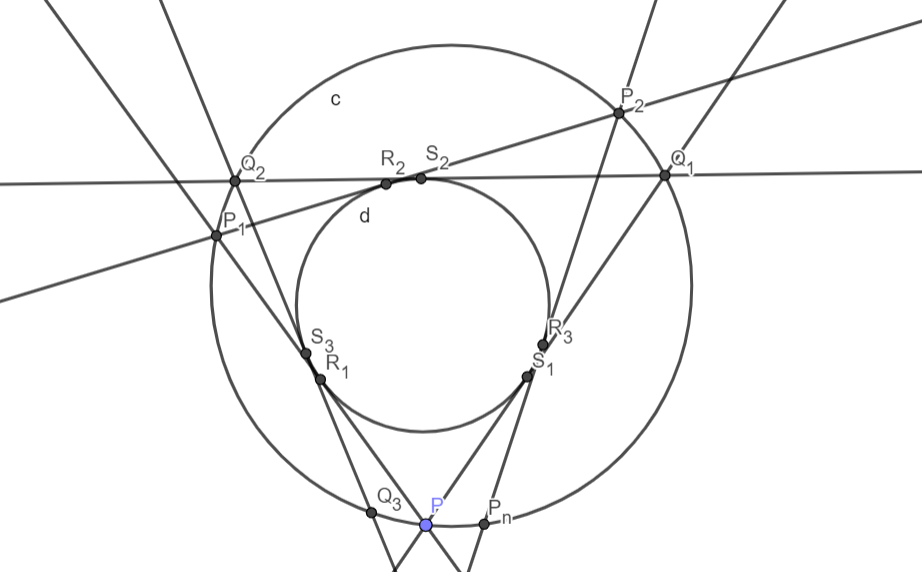
\includegraphics[width=0.9\textwidth]{kepek/poncelet.png}
    \end{figure}


    Define distinct points $P_0,\ldots, P_n\in C$ such that $P_{i-1}P_i$ is tangent to $D$ for every $i=1,\ldots,n$, $P_0=P$, and $P_0P_1$ is at the 'left' side of $D$.

    The statement is equivalent to $P_0=P_n$

    We can similarly define $Q_0,\ldots, Q_n$, but $Q_0Q_1$ is at the 'right' side of $D$.

    Let $R_1,\ldots, R_n$ be the tangency points of $P_0P_1,\ldots, P_{n-1}P_n$ on $D$.
    Similarly we define $S_i$ to be the tangency point of $Q_{i-1}Q_i$ on $D$.

    Now we fix $C$, $D$, and animate $P$ so that it is a degree 2 polynomial moving point on $C$.

    $R_1S_1$ is the polar of $P$ to $D$, so it is also of degree 2.

    A polynomial moving line of degree 2 intersects $D$ at a square root point pair of degree 2.

    The polar of $(R_1,S_1)$ is $(P_0P_1,Q_0Q_1)$, so it is also degree 2.

    By the inverse of Sqrt Mászó-tétel $\frac{\deg (P_1,Q_1)+2}{2}=2$, so $\deg (P_1,Q_1)=2$.

    And so on, we iterate sqrt pole-polar theorems and sqrt inverse Mászó-theorems to get that every square root point/line pair on the figure is of degree 2.

    Now $(P_n, Q_n)$ is of degree 2, and $(P,P)$ is of degree 2.

    So the degree of the statement "$P=P_n$ or $P=Q_n$" is $\frac{2+2}{2}=2$.

    This means that if "$P=P_n$ or $P=Q_n$" happens more than 4 times, it is always true, and when they are both true, that counts as 2.

    Luckily $P=P_n \iff P=Q_n$. So it is sufficient to find 3 cases when both statements are true.

    The condition of the porism states that there exists a good $n$-gon, so when $P$ is at the vertices of the $n$-gon we instantly have $n$ cases when both $P=P_n$ and $P=Q_n$.

    $n\geq3$, so we are finished.
\end{proof}


\section{Length and area}

\subsection{Length of segments}

\begin{definition}
     The complex length-square $|AB|^2$ of segment $AB$ is defined to be $(a_x-b_x)^2+(a_y-b_y)^2$, this is a complex number.
\end{definition}

\begin{theorem}
    Let $A$ and $B$ be polynomial moving points. Then the complex length-square $|AB|^2$ of segment $AB$ is a polynomial quantity with degree
    $$\deg |AB|^2=2\deg A+2\deg B-$$
    $$-\sum_{t\in\cc\pp^1}\min\Big(\ord(A,B,\alpha_i\text{ collinear})+\ord(A,B,\alpha_{-i}\text{ collinear}),$$
    $$2\ord(A\in \text{ideal line})+2\ord(B\in \text{ideal line})\Big)$$
\end{theorem}
\begin{remark}
    The multiplicity $\ord(A,B,C\text{ collinear})$ is the order of zero of the area of the triangle $ABC$ according to any chart containing $A$, $B$ and $C$. (see ~\ref{3pmul})

    The multiplicity $\ord(P\in l)$ is the order of zero of the distance of $P$ from $l$ according to any chart containing $P$. (see ~\ref{plmul})
\end{remark}
\begin{remark}
    If either $A$ or $B$ is at one of the circle points (say $A$), then we can reduce the degree by at least one, since then $"A\in \text{ideal line}"$ is true, and $"A,B,\alpha_i\text{ collinear}"$ is also true (or with $\alpha{-i}$).

    If both $A$ and $B$ are ideal points, then we can reduce by at least 2, since then both $"A,B,\alpha_i\text{ collinear}"$ and $"A,B,\alpha_{-i}\text{ collinear}"$ are true, and also $2\ord(A\in \text{ideal line})+2\ord(B\in \text{ideal line})\ge 4$, so we are good on that side by far.
\end{remark}
\begin{proof}
$A=(a_0:a_1:a_2)$ and $B=(b_0:b_1:b_2)$.




With euclidean coordinates
$$|AB|^2=\left(\frac{a_0}{a_2}-\frac{b_0}{b_2}\right)^2+\left(\frac{a_1}{a_2}-\frac{b_1}{b_2}\right)^2=\frac{(a_0b_2-b_0a_2)^2+(a_1b_2-b_1a_2)^2}{(a_2b_2)^2}$$
So
with homogeneous coordinates in $\cc\pp^1$ this is
$$|AB|^2=\big((a_0b_2-b_0a_2)^2+(a_1b_2-b_1a_2)^2:(a_2b_2)^2\big)$$
Now use lemma ~\ref{polyconst}:

These are degree $2\deg A+2\deg B$ polynomials, and we have to subtract $\sum_{t\in\cc\pp^1}\ord\Big(|AB|^2=(0,0)\Big)$ from this to get the degree of $|AB|^2$
$$\ord\Big(|AB|^2=(0,0)\Big)\overset{\text{by def}}{=}\min\Big(\ord\big((a_0b_2-b_0a_2)^2+(a_1b_2-b_1a_2)^2\big), \ord\big((a_2b_2)^2\big)\Big)=$$
$$\min\Big(\ord\big([-i(a_0b_2-b_0a_2)+(a_1b_2-b_1a_2)][i(a_0b_2-b_0a_2)+(a_1b_2-b_1a_2)]\big), \ord\big((a_2b_2)^2\big)\Big)=$$
$$\min\Big(\ord\big(-i(a_0b_2-b_0a_2)+(a_1b_2-b_1a_2)\big)+\ord\big(i(a_0b_2-b_0a_2)+(a_1b_2-b_1a_2)\big), 2\ord(a_2)+2\ord(b_2)\Big)=$$
$$\min\left(\ord\left(\det
\begin{bmatrix}
a_0 & a_1 & a_2 \\
b_0 & b_1 & b_2 \\
1 & i & 0
\end{bmatrix}
\right)+\ord\left(\det
\begin{bmatrix}
a_0 & a_1 & a_2 \\
b_0 & b_1 & b_2 \\
1 & -i & 0
\end{bmatrix}
\right),
2\ord((a_0,a_1,a_2)\cdot(0,0,1))+2\ord((b_0,b_1,b_2)\cdot(0,0,1))\right)=$$
$$\overset{\text{see below}}{=}\min\Big(\ord(A,B,\alpha_i\text{ collinear})+\ord(A,B,\alpha_{-i}\text{ collinear}), 2\ord(A\in \text{ideal line})+2\ord(B\in \text{ideal line})\Big)$$

According to ~\ref{3pmul}, $\ord(A,B,\alpha_i\text{ collinear})=\ord\left(\det
\begin{bmatrix}
a_0 & a_1 & a_2 \\
b_0 & b_1 & b_2 \\
1 & i & 0
\end{bmatrix}
\right)$

Also according to ~\ref{plmul}, $\ord(A\in \text{ideal line})=\ord\big((a_0,a_1,a_2)\cdot(0,0,1)\big)=\ord(a_2)$, where this is a dot product.
\end{proof}


%%%%%%%%%%%%%%%%%%%%%%%%%%%%%%%%%%%%%%%%%%%%%%%%%%


\bibliographystyle{plain}
\bibliography{forrasok}




\end{document}
